\documentclass[xetex,10pt,mathserif,handout]{beamer}

\usetheme{Boadilla}
\usecolortheme{seahorse}

\usefonttheme{professionalfonts}
\usepackage{fontspec}
\usepackage{xunicode}
\usepackage{xltxtra}
\setmainfont[Ligatures={Common,TeX}, Scale=0.95]{Myriad Pro}
\setsansfont[Ligatures={Common,TeX}, Scale=0.95]{Myriad Pro}

\usepackage{media9}
\usepackage{grfext}\PrependGraphicsExtensions*{.png,.PNG}


%%
\usepackage{mathtools}
\usepackage{xspace}
\usepackage{makecell}
\usepackage{msthpres}
\usepackage{pdfpages} 
%%

\usepackage{tikz}
\usetikzlibrary{arrows,positioning,shapes,fit}
\usepackage{pgfplots}
\usepgfplotslibrary{fillbetween,colormaps}
\newlength\figureheight
\newlength\figurewidth

% presentation stuff
\newcommand{\sig}[2]{%
\begin{tabular}{r}
#1\\[-0.7em]
{\tiny \color{darkgray}\it #2\hspace{0.5em}}
\end{tabular}}

\newcommand{\qauth}[1]{{\footnotesize\par\normalfont\hfill---\ \emph{#1}\par}}

\newcommand{\qcite}[1]{{\small\color{gray}[#1]}}

% math stuff
\newcommand{\defeq}{\vcentcolon=}
\newcommand{\LLC}{$L$-Lipschitz continuous}
\newcommand{\Reps}{R_{\epsilon}}
\newcommand{\Rbeps}{\bar{R}_{\epsilon}}
\newcommand{\Ro}{R_{0}}
\newcommand{\Rbo}{\bar{R}_{0}}
\newcommand{\xb}{\hat{\*x}}
\newcommand{\smid}{\ \middle\vert\ }
\newcommand{\bigsmid}{\ \big\vert\ }
\newcommand{\setdef}[2]{\left\{ #1 \smid #2 \right\}}
\newcommand{\bigsetdef}[2]{\big\{ #1 \bigsmid #2 \big\}}

\usepackage{xspace}
\newcommand{\algo}{{\sc\textsf{SafeOpt}}\xspace}
\newcommand{\gpucb}{{\sc\textsf{GP-UCB}}\xspace}
\newcommand{\localucb}{{\sc\textsf{Safe-UCB}}\xspace}

% Colored sets
\newcommand{\cst}{{\color{cyan!70!black}$S_t$}\xspace}
\newcommand{\ccst}{{\color{cyan!70!black}S_t}\xspace}
\newcommand{\cgt}{{\color{lime!70!black}$G_t$}\xspace}
\newcommand{\ccgt}{{\color{lime!70!black}G_t}\xspace}
\newcommand{\cmt}{{\color{orange!70!black}$M_t$}\xspace}
\newcommand{\ccmt}{{\color{orange!70!black}M_t}\xspace}
\newcommand{\crbo}{{\color{magenta!70!black}$\Rbo(S_0)$}\xspace}
\newcommand{\crbeps}{{\color{magenta!70!black}$\Rbeps(S_0)$}\xspace}
\newcommand{\ccrbeps}{{\color{magenta!70!black}\Rbeps(S_0)}\xspace}

\title[Safe Gaussian Process Optimization]
{Safe Exploration for Optimization with Gaussian Processes}

\author[Alkis Gotovos]{
\vspace{1in}
\normalsize
\parbox{1in}{Yanan Sui\\{\footnotesize Caltech}}\and
\parbox{1in}{Alkis Gotovos\\{\footnotesize ETH Zurich}}\and
\parbox{1in}{Joel W. Burdick\\{\footnotesize Caltech}}\and
\parbox{1in}{Andreas Krause\\{\footnotesize ETH Zurich}}
}

\date[May 4, 2015]{
\begin{center}
{\normalsize
ICML '15
}
\end{center}
}

\begin{document}

\setbeamercolor{background canvas}{bg=}
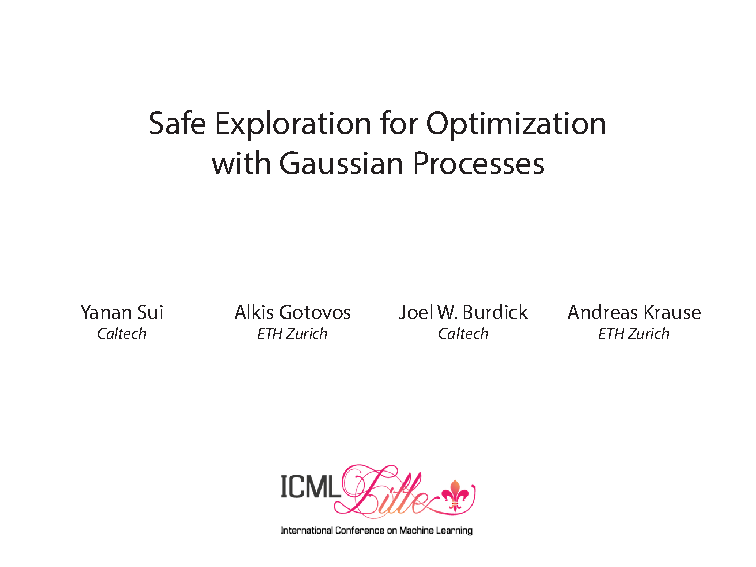
\includepdf[pages={1}]{title.pdf}

\section{Motivation}

\begin{frame}{Better safe than sorry}
\begin{center}
\sig{
\includemedia[
width=4.7in,height=2.655in,
addresource=figures/robot.mp4,
activate=pageopen,
flashvars={
autoPlay=true
&source=figures/robot.mp4
&loop=true % loop video
&scaleMode=letterbox % preserve aspect ratio while scaling the video
}
]{}{VPlayer.swf}
}{youtube.com/user/mattessons}
\end{center}
\end{frame}

\begin{frame}{Therapeutic spinal cord stimulation}
\begin{columns}[c]
\column{0.45\textwidth}
\centering
\sig{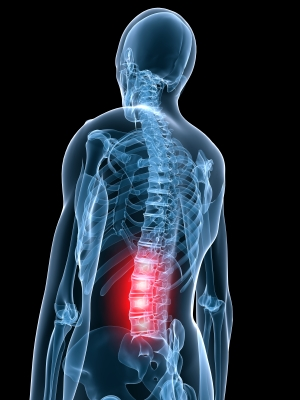
\includegraphics[width=2in]{figures/spinal1.jpg}}{girardgibbs.com}

\column{0.55\textwidth}
\centering
\sig{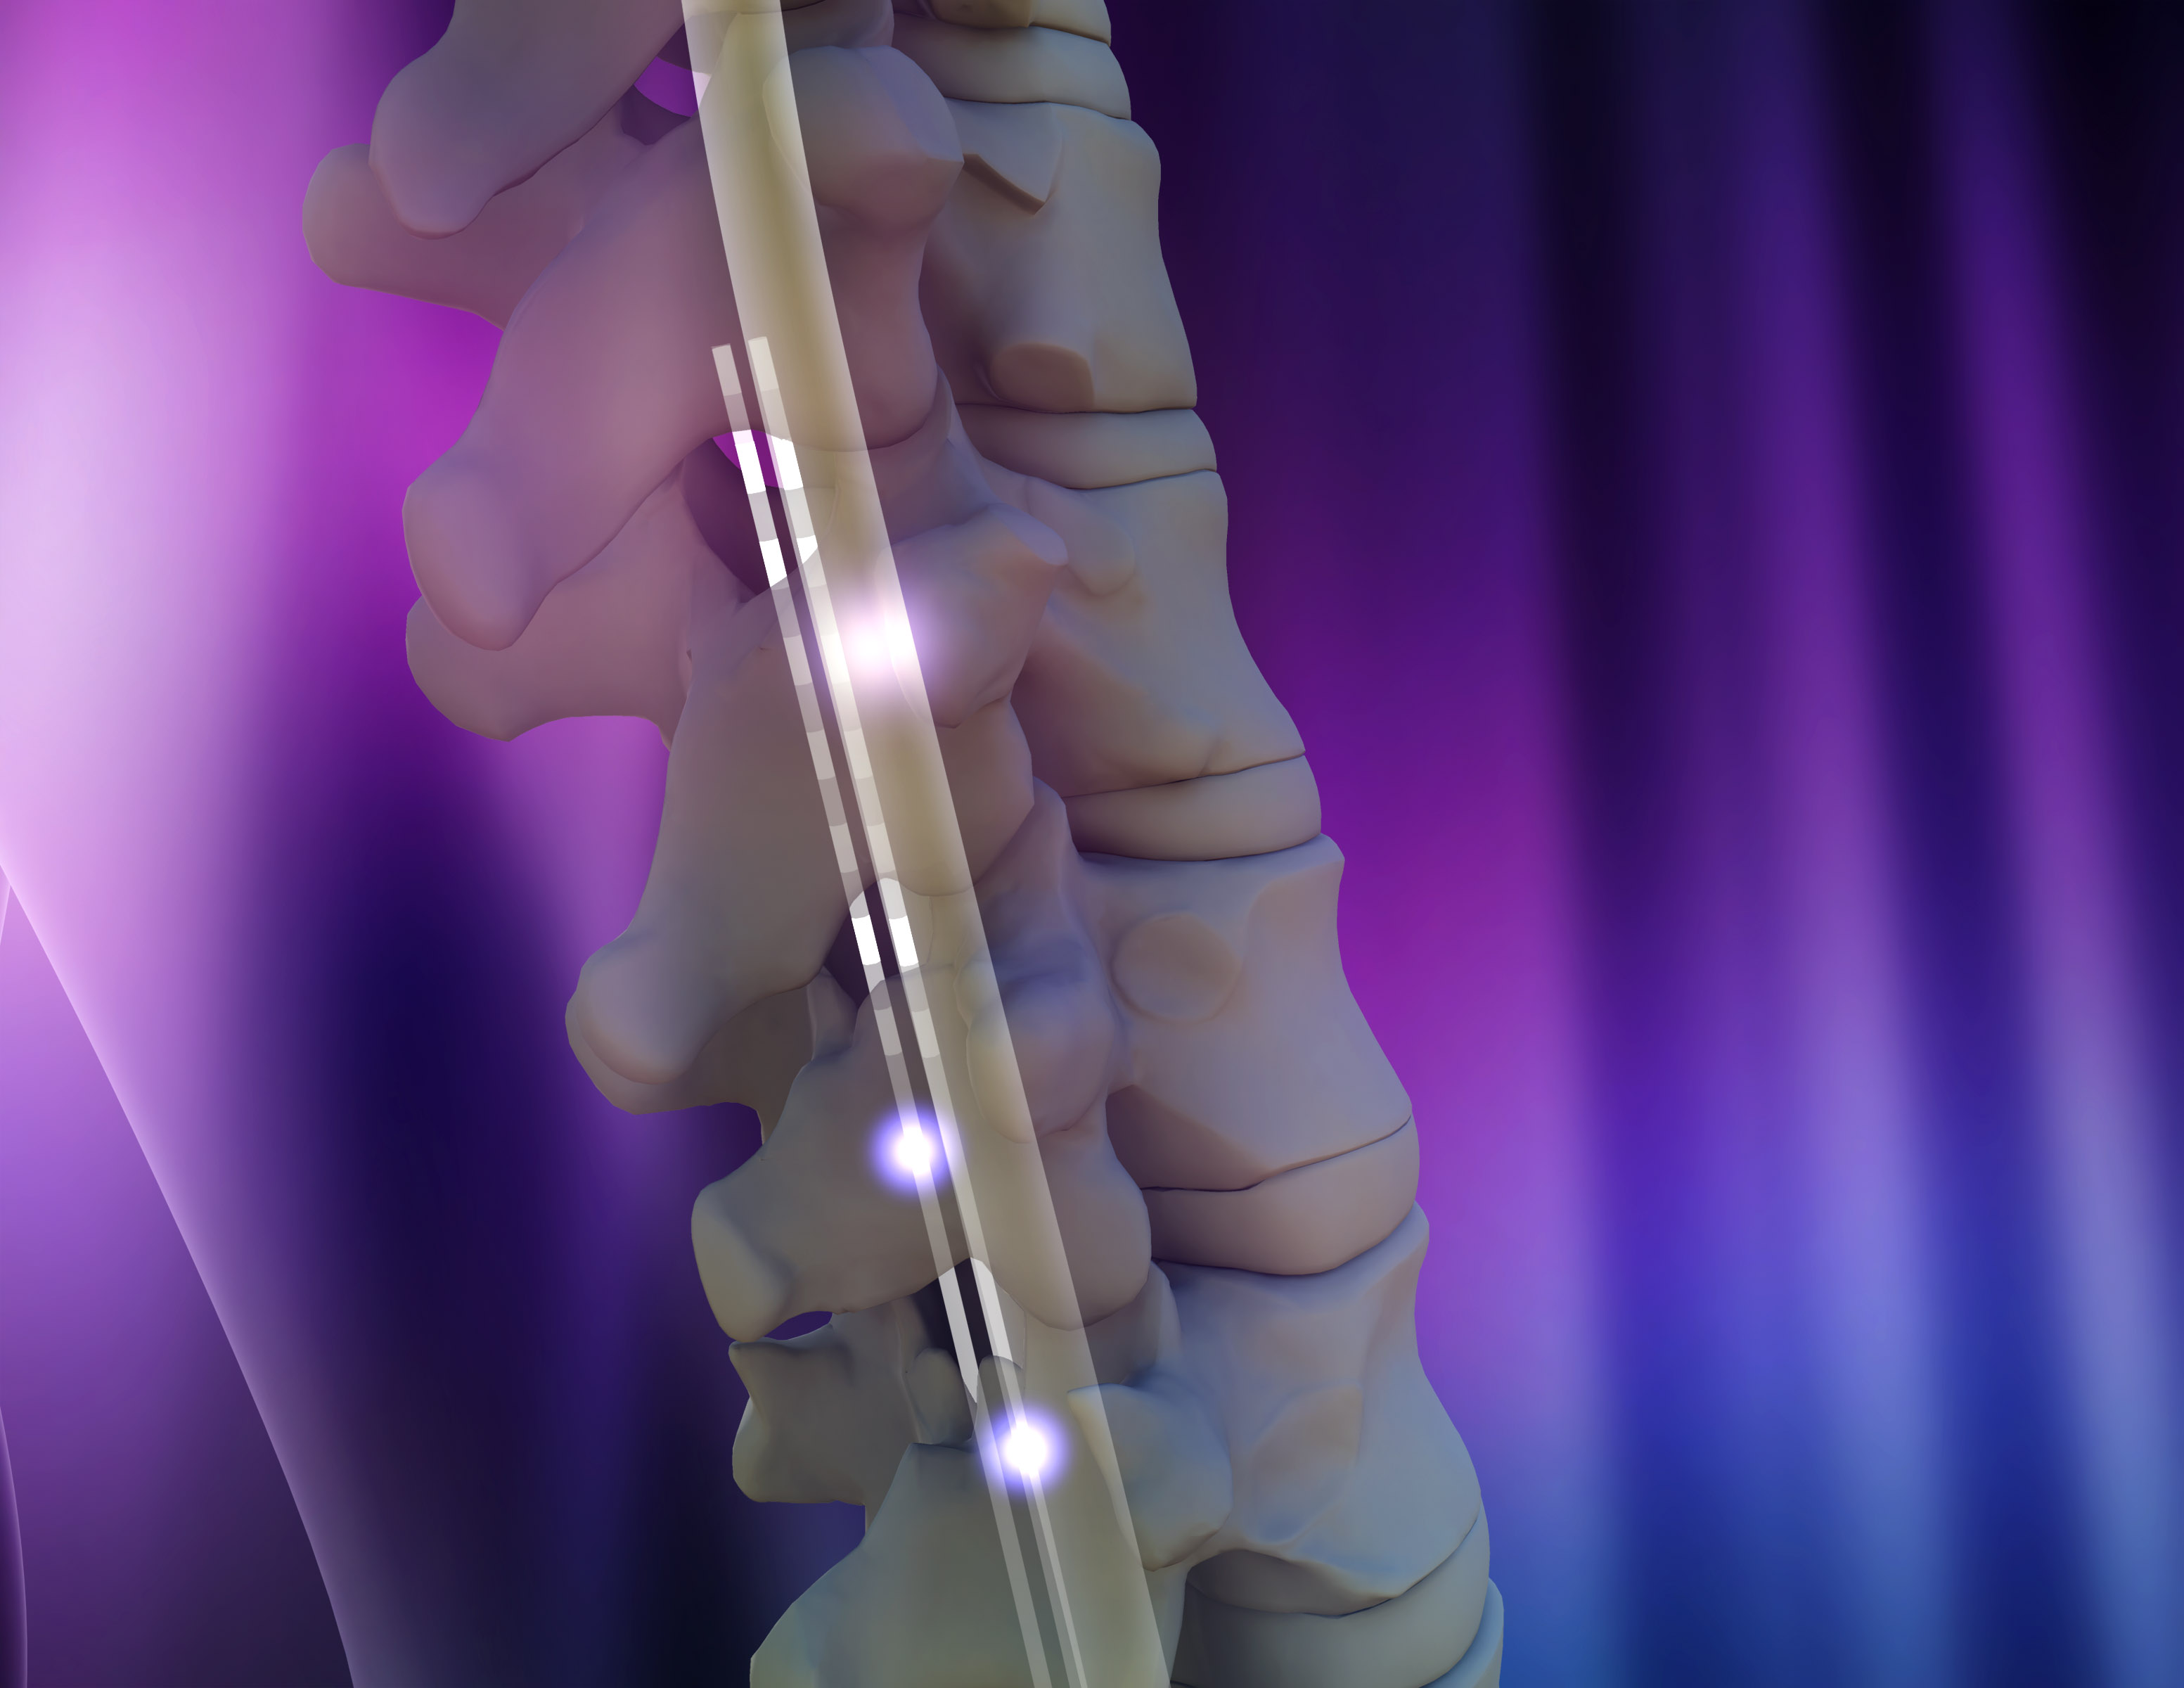
\includegraphics[width=2.37in]{figures/spinal2.jpg}}{sjm.com}
\begin{itemize}
\item Find electrode configurations that maximize muscle activity
\vspace{0.5em}
\item Bad configurations may cause pain or have negative effects on treatment
\end{itemize}
\end{columns}
\end{frame}

%\begin{frame}{Movie recommendation}
%\centering
%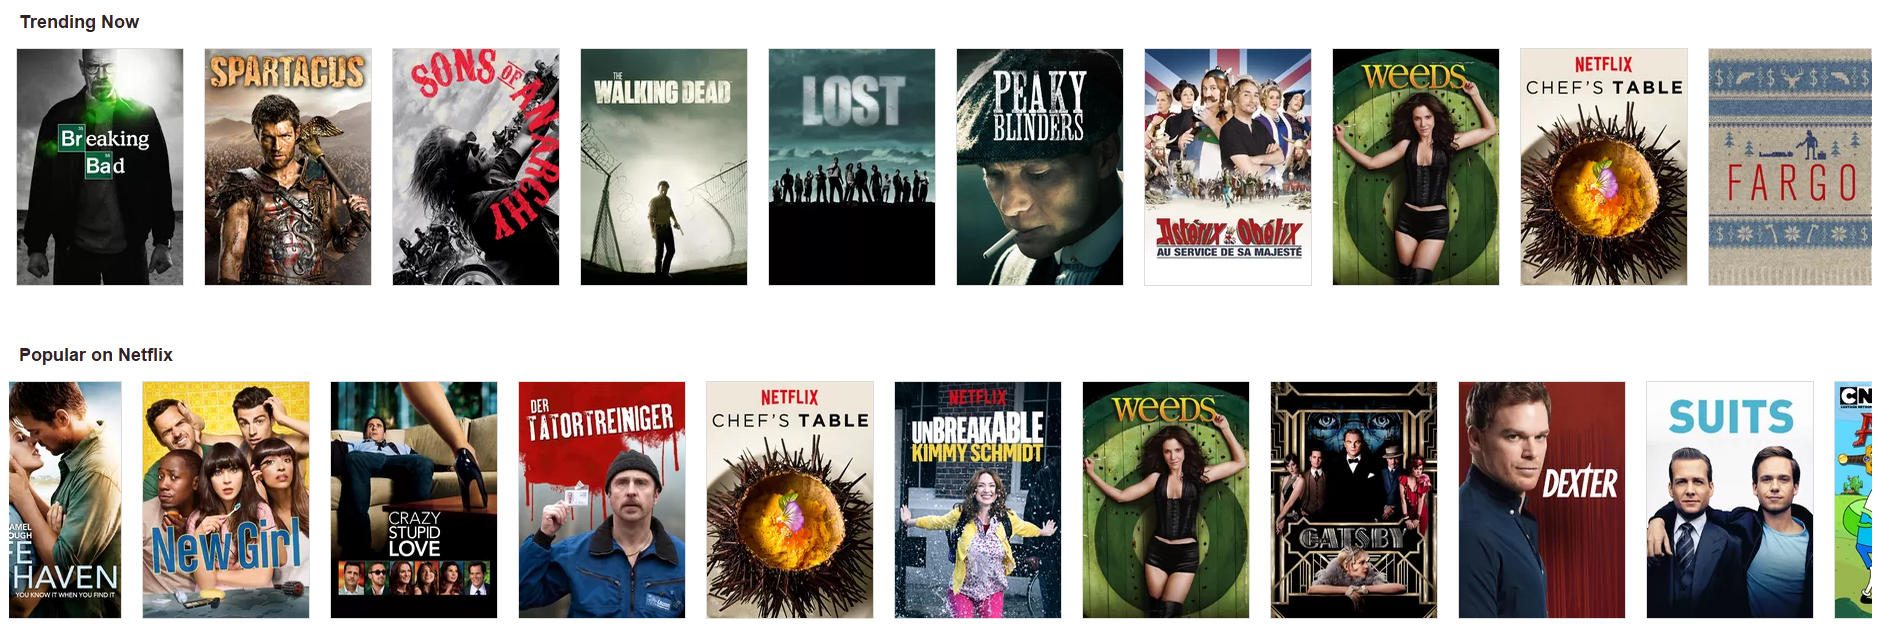
\includegraphics[width=4.5in]{figures/netflix.png}
%\vspace{2em}
%\begin{itemize}
%\item Explore the movie space to discover each user's taste profile
%\vspace{0.5em}
%\item Bad recommendations may cause user dissatisfaction
%\end{itemize}
%\end{frame}

\begin{frame}{Goal}
\centering
\large
Optimize an unknown reward function via sequential sampling\\[1em]
AND\\[1em]
remain ``safe'' throughout the process.
\end{frame}

\begin{frame}{Problem statement}
\begin{itemize}
\item<1-> Finite decision set $D$
\vspace{0.5em}
\item<1-> Unknown reward function $f : D \to \mathbb{R}$
\vspace{0.5em}
\item<2-> Safety threshold $h \in \mathbb{R}$
\vspace{0.5em}
\item<4-> Seed set $S_0$ of safe decisions ($\forall x \in S_0,\ f(x) \geq h$)
\end{itemize}

\only<1>{
\vspace{1em}
\centering
\setlength\figurewidth{4in}
\setlength\figureheight{2.5in}
\begin{tikzpicture}

\begin{axis}[
width=\figurewidth,
height=\figureheight,
xmin=0, xmax=10,
ymin=-2, ymax=3.5,
xticklabels={,,},
yticklabels={,,},
major tick length=0pt,
clip=false
]

\addplot[
  gray,
  solid,
  line width=1.3pt
]
table [col sep=comma] {matlab/ftrue.csv};

\node at (axis cs:-0.3,-0.3) [anchor=south,minimum size=16pt] {\color{white}$h$};

\end{axis}

\end{tikzpicture}

}

\only<2>{
\vspace{1em}
\centering
\setlength\figurewidth{4in}
\setlength\figureheight{2.5in}
\begin{tikzpicture}

\begin{axis}[
width=\figurewidth,
height=\figureheight,
xmin=0, xmax=10,
ymin=-2, ymax=3.5,
xticklabels={,,},
yticklabels={,,},
major tick length=0pt,
clip=false
]

\addplot [
  magenta!50!darkgray,
  line width=1pt,
  densely dashed
]
table [col sep=comma] {matlab/hp.csv};

\addplot[
  gray,
  solid,
  line width=1.3pt
]
table [col sep=comma] {matlab/ftrue.csv};

\node at (axis cs:-0.3,-0.3) [anchor=south,minimum size=16pt] {$h$};

\end{axis}

\end{tikzpicture}

}

\only<3>{
\vspace{1em}
\centering
\setlength\figurewidth{4in}
\setlength\figureheight{2.5in}
\begin{tikzpicture}

\begin{axis}[
width=\figurewidth,
height=\figureheight,
xmin=0, xmax=10,
ymin=-2, ymax=3.5,
xticklabels={,,},
yticklabels={,,},
major tick length=0pt,
clip=false
]

\addplot [
  magenta!50!darkgray,
  line width=1pt,
  densely dashed
]
table [col sep=comma] {matlab/hp.csv};

\addplot[
  gray,
  solid,
  line width=1.3pt
]
table [col sep=comma] {matlab/ftrue.csv};

\addplot [
darkgray,
densely dashed,
line width=0.5pt,
]
coordinates{(0.97,-1.9)(0.97,0)};

\addplot [
darkgray,
densely dashed,
line width=0.5pt,
]
coordinates{(2.48,-1.9)(2.48,0)};

\addplot [
darkgray,
densely dashed,
line width=0.5pt,
]
coordinates{(6.86,-1.9)(6.86,0)};

\addplot [
darkgray,
densely dashed,
line width=0.5pt,
]
coordinates{(8.77,-1.9)(8.77,0)};

\addplot[
only marks,
mark=square*,
cyan!70!black,
mark size=2
]
table [col sep=comma] {matlab/fsafe.csv};

\addplot[
only marks,
mark=square*,
red!70!black,
mark size=2
]
table [col sep=comma] {matlab/funsafe.csv};

\node at (axis cs:-0.3,-0.3) [anchor=south,minimum size=16pt] {$h$};

\end{axis}

\end{tikzpicture}

}

\only<4>{
\vspace{1em}
\centering
\setlength\figurewidth{4in}
\setlength\figureheight{2.5in}
\begin{tikzpicture}

\begin{axis}[
width=\figurewidth,
height=\figureheight,
xmin=0, xmax=10,
ymin=-2, ymax=3.5,
xticklabels={,,},
yticklabels={,,},
major tick length=0pt,
clip=false
]

\addplot [
  magenta!50!darkgray,
  line width=1pt,
  densely dashed
]
table [col sep=comma] {matlab/hp.csv};

\addplot[
  gray,
  solid,
  line width=1.3pt
]
table [col sep=comma] {matlab/ftrue.csv};

\addplot [
darkgray,
densely dashed,
line width=0.5pt,
]
coordinates{(0.97,-1.9)(0.97,0)};

\addplot [
darkgray,
densely dashed,
line width=0.5pt,
]
coordinates{(2.48,-1.9)(2.48,0)};

\addplot [
darkgray,
densely dashed,
line width=0.5pt,
]
coordinates{(6.86,-1.9)(6.86,0)};

\addplot [
darkgray,
densely dashed,
line width=0.5pt,
]
coordinates{(8.77,-1.9)(8.77,0)};

\addplot[
only marks,
mark=square*,
cyan!70!black,
mark size=2
]
table [col sep=comma] {matlab/fsafe.csv};

\addplot[
only marks,
mark=square*,
red!70!black,
mark size=2
]
table [col sep=comma] {matlab/funsafe.csv};

\addplot[
lime!50!darkgray,
only marks,
mark=*,
mark size=2.5
]
table [col sep=comma] {matlab/s0.csv};

\addplot[
lime!50!darkgray,
only marks,
mark=*,
mark size=2.5
]
table [col sep=comma] {matlab/cert1-s0.csv};

\node at (axis cs:-0.3,-0.3) [anchor=south,minimum size=16pt] {$h$};

\end{axis}

\end{tikzpicture}

}
\end{frame}

\begin{frame}{Problem statement}

Sequential sampling
\vspace{0.5em}
\begin{itemize}
\item For $t = 1, 2, \ldots$
  \vspace{0.5em}
  \begin{itemize}
    \item select $x_t \in D$
    \vspace{0.5em}
    \item observe $f(x_t) + n_t$
  \end{itemize}
\end{itemize}

\invisible<-1>{
\alt<3>{
\vspace{3em}
Goal
\vspace{0.5em}
\begin{itemize}
\item Find $x^* \in \argmax_{x\in D}f(x)$
\vspace{0.5em}
\item \fcolorbox{blue}{blue!40!white}{\makebox{Remain safe: $\forall t \geq 1,\ f(x_t) \geq h$}}
\end{itemize}
}{
\vspace{3em}
Goal
\vspace{0.5em}
\begin{itemize}
\item Find $x^* \in \argmax_{x\in D}f(x)$
\vspace{0.5em}
\item Remain safe: $\forall t \geq 1,\ f(x_t) \geq h$
\end{itemize}
}}
\end{frame}

\begin{frame}{Related work}
\begin{itemize}
  \item<1-> Bayesian optimization: function evaluation is expensive
  \vspace{2em}
  \item<2-> Various proposed criteria, e.g.,
    \vspace{0.5em}
    \begin{itemize}
      \item Expected improvement \qcite{Mockus et al., 1974}
      \vspace{0.5em}
      \item UCB \qcite{Auer, 2002} \qcite{Srinivas et al., 2010}
    \end{itemize}
  \vspace{2em}
  \item<3-> Related variants
    \vspace{0.5em}
    \begin{itemize}
      \item Level set estimation \qcite{Gotovos et al., 2013}
      \vspace{0.5em}
      \item Bayesian optimization with constraints \qcite{Gardner et al., 2014}
    \end{itemize}
  \vspace{2em}
  \item<4-> Gaussian processes popular for modeling the unknown function
\end{itemize}
\end{frame}

\begin{frame}{Gaussian process regression}
\centering
\setlength\figurewidth{5in}
\setlength\figureheight{3.5in}
\begin{tikzpicture}

\begin{axis}[
width=\figurewidth,
height=\figureheight,
xmin=0, xmax=10,
ymin=-2, ymax=3.5,
xticklabels={,,},
yticklabels={,,},
major tick length=0pt
]

\addplot[
  gray,
  solid,
  line width=1.3pt
]
table [col sep=comma] {matlab/ftrue.csv};

\end{axis}

\end{tikzpicture}

\end{frame}

\begin{frame}{Gaussian process regression}
\centering
\setlength\figurewidth{5in}
\setlength\figureheight{3.5in}
\begin{tikzpicture}

\begin{axis}[
width=\figurewidth,
height=\figureheight,
xmin=0, xmax=10,
ymin=-2, ymax=3.5,
xticklabels={,,},
yticklabels={,,},
major tick length=0pt
]

\addplot [
name path=A,
draw=olive!20!lightgray,
draw=none
]
table [col sep=comma] {matlab/gp-0-lt.csv};

\addplot [
name path=B,
draw=olive!20!lightgray,
draw=none
]
table [col sep=comma] {matlab/gp-0-ut.csv};

\addplot[lime!30!gray, opacity=0.5] fill between[of=A and B];

\addplot[
  gray,
  solid,
  line width=1.3pt
]
table [col sep=comma] {matlab/ftrue.csv};

\addplot[
olive!50!darkgray,
densely dotted,
line width=1.2pt
]
table [col sep=comma] {matlab/gp-0-mt.csv};

\end{axis}

\end{tikzpicture}

\end{frame}

\begin{frame}{Gaussian process regression}
\centering
\setlength\figurewidth{5in}
\setlength\figureheight{3.5in}
\begin{tikzpicture}

\begin{axis}[
width=\figurewidth,
height=\figureheight,
xmin=0, xmax=10,
ymin=-2, ymax=3.5,
xticklabels={,,},
yticklabels={,,},
major tick length=0pt
]

\addplot [
name path=A,
draw=olive!20!lightgray,
draw=none
]
table [col sep=comma] {matlab/gp-1-lt.csv};

\addplot [
name path=B,
draw=olive!20!lightgray,
draw=none
]
table [col sep=comma] {matlab/gp-1-ut.csv};

\addplot[lime!30!gray, opacity=0.5] fill between[of=A and B];

\addplot[
  gray,
  solid,
  line width=1.3pt
]
table [col sep=comma] {matlab/ftrue.csv};

\addplot[
only marks,
mark=x,
lime!30!black,
mark size=3.5,
line width=1.4pt,
opacity=0.8
]
table [col sep=comma] {matlab/gp-1-train.csv};

\addplot[
olive!50!darkgray,
densely dotted,
line width=1.2pt
]
table [col sep=comma] {matlab/gp-1-mt.csv};

\end{axis}

\end{tikzpicture}

\end{frame}

\begin{frame}{Gaussian process regression}
\centering
\setlength\figurewidth{5in}
\setlength\figureheight{3.5in}
\begin{tikzpicture}

\begin{axis}[
width=\figurewidth,
height=\figureheight,
xmin=0, xmax=10,
ymin=-2, ymax=3.5,
xticklabels={,,},
yticklabels={,,},
major tick length=0pt
]

\addplot [
name path=A,
draw=olive!20!lightgray,
draw=none
]
table [col sep=comma] {matlab/gp-2-lt.csv};

\addplot [
name path=B,
draw=olive!20!lightgray,
draw=none
]
table [col sep=comma] {matlab/gp-2-ut.csv};

\addplot[lime!30!gray, opacity=0.5] fill between[of=A and B];

\addplot[
  gray,
  solid,
  line width=1.3pt
]
table [col sep=comma] {matlab/ftrue.csv};

\addplot[
only marks,
mark=x,
lime!30!black,
mark size=3.5,
line width=1.4pt,
opacity=0.8
]
table [col sep=comma] {matlab/gp-2-train.csv};

\end{axis}

\end{tikzpicture}

\end{frame}

\begin{frame}{Gaussian process regression}
\centering
\setlength\figurewidth{5in}
\setlength\figureheight{3.5in}
\begin{tikzpicture}

\begin{axis}[
width=\figurewidth,
height=\figureheight,
xmin=0, xmax=10,
ymin=-2, ymax=3.5,
xticklabels={,,},
yticklabels={,,},
major tick length=0pt,
clip=false
]

\addplot [
name path=A,
draw=olive!20!lightgray,
draw=none
]
table [col sep=comma] {matlab/gp-3-lt.csv};

\addplot [
name path=B,
draw=olive!20!lightgray,
draw=none
]
table [col sep=comma] {matlab/gp-3-ut.csv};

\addplot[lime!30!gray, opacity=0.5] fill between[of=A and B];

\addplot[
  gray,
  solid,
  line width=1.3pt
]
table [col sep=comma] {matlab/ftrue.csv};

\addplot[
only marks,
mark=x,
lime!30!black,
mark size=3.5,
line width=1.4pt,
opacity=0.8
]
table [col sep=comma] {matlab/gp-3-train.csv};

\addplot[
olive!50!darkgray,
densely dashed,
line width=1.7pt
]
table [col sep=comma] {matlab/gp-3-mt.csv};

\end{axis}

\end{tikzpicture}

\end{frame}

\begin{frame}{Gaussian process regression}
\centering
\setlength\figurewidth{5in}
\setlength\figureheight{3.5in}
\begin{tikzpicture}

\begin{axis}[
width=\figurewidth,
height=\figureheight,
xmin=0, xmax=10,
ymin=-2, ymax=3.5,
xticklabels={,,},
yticklabels={,,},
major tick length=0pt,
clip=false
]

\addplot [
name path=A,
draw=olive!20!lightgray,
draw=none
]
table [col sep=comma] {matlab/gp-3-lt.csv};

\addplot [
name path=B,
draw=olive!20!lightgray,
draw=none
]
table [col sep=comma] {matlab/gp-3-ut.csv};

\addplot[lime!30!gray, opacity=0.5] fill between[of=A and B];

\addplot[
  gray,
  solid,
  line width=1.3pt
]
table [col sep=comma] {matlab/ftrue.csv};

\addplot[
only marks,
mark=x,
lime!30!black,
mark size=3.5,
line width=1.4pt,
opacity=0.8
]
table [col sep=comma] {matlab/gp-3-train.csv};

\addplot [
color=gray,
densely dotted,
line width=1pt,
forget plot
]
coordinates{
(3.9698,-2)(3.9698,-0.6618)
};

\addplot [
color=black,
solid,
line width=1.5pt,
mark=-,
mark size=3pt
]
coordinates{
(3.9698,-0.6618)(3.9698,1.2188)
};

\node at (axis cs:4.3,1.2) [anchor=south,minimum size=16pt] {\large$u_t(x)$};
\node at (axis cs:4.5,-1) [anchor=south,minimum size=16pt] {\large$\ell_t(x)$};
\node at (axis cs:3.9698,-2.4) [anchor=south,minimum size=16pt] {\large$x$};

\end{axis}

\end{tikzpicture}

\end{frame}

\begin{frame}{GP-UCB}
\begin{itemize}
\item<1-> Use upper confidence bounds for optimistic sampling
\vspace{1em}
\item<2-> $x_t = \argmax_{x \in D}u_t(x)$\\[1em]
  \centering
  \setlength\figurewidth{4in}
  \setlength\figureheight{2.5in}
  \begin{tikzpicture}

\begin{axis}[
width=\figurewidth,
height=\figureheight,
xmin=0, xmax=10,
ymin=-2, ymax=3.5,
xticklabels={,,},
yticklabels={,,},
major tick length=0pt,
clip=false
]

\addplot [
name path=A,
draw=olive!20!lightgray,
draw=none
]
table [col sep=comma] {matlab/gp-3-lt.csv};

\addplot [
name path=B,
draw=olive!20!lightgray,
draw=none
]
table [col sep=comma] {matlab/gp-3-ut.csv};

\addplot[lime!30!gray, opacity=0.5] fill between[of=A and B];

\addplot[
  gray,
  solid,
  line width=1.3pt
]
table [col sep=comma] {matlab/ftrue.csv};

\addplot[
only marks,
mark=x,
lime!30!black,
mark size=3.5,
line width=1.4pt,
opacity=0.8
]
table [col sep=comma] {matlab/gp-3-train.csv};

\addplot[
olive!50!gray,
solid,
line width=1.7pt
]
table [col sep=comma] {matlab/gp-3-ut.csv};

\end{axis}

\end{tikzpicture}

\vspace{0.5em}
\item<3-> Sublinear regret under suitable conditions on $f$ \qcite{Srinivas et al., 2010}
\end{itemize}
\end{frame}

\begin{frame}{GP-UCB example ($t = 0$)}
\centering
\setlength\figurewidth{5in}
\setlength\figureheight{3.5in}
\begin{tikzpicture}

\begin{axis}[
width=\figurewidth,
height=\figureheight,
xmin=0, xmax=10,
ymin=-2, ymax=3.5,
xticklabels={,,},
yticklabels={,,},
major tick length=0pt
]

\addplot [
name path=A,
draw=olive!20!lightgray,
draw=none
]
table [col sep=comma] {matlab/gpucb-0-lt.csv};

\addplot [
name path=B,
draw=olive!20!lightgray,
draw=none
]
table [col sep=comma] {matlab/gpucb-0-ut.csv};

\addplot[lime!30!gray, opacity=0.5] fill between[of=A and B];

\addplot [
  magenta!50!darkgray,
  line width=1pt,
  densely dashed
]
table [col sep=comma] {matlab/hp.csv};

\addplot[
  gray,
  solid,
  line width=1.3pt
]
table [col sep=comma] {matlab/ftrue.csv};

\end{axis}

\end{tikzpicture}

\end{frame}

\begin{frame}{GP-UCB example ($t = 5$)}
\centering
\setlength\figurewidth{5in}
\setlength\figureheight{3.5in}
\begin{tikzpicture}

\begin{axis}[
width=\figurewidth,
height=\figureheight,
xmin=0, xmax=10,
ymin=-2, ymax=3.5,
xticklabels={,,},
yticklabels={,,},
major tick length=0pt
]

\addplot [
  name path=A,
  draw=olive!20!lightgray,
  draw=none
]
table [col sep=comma] {matlab/gpucb-5-lt.csv};

\addplot [
  name path=B,
  draw=olive!20!lightgray,
  draw=none
]
table [col sep=comma] {matlab/gpucb-5-ut.csv};

\addplot[lime!30!gray, opacity=0.5] fill between[of=A and B];

\addplot [
  magenta!50!darkgray,
  line width=1pt,
  densely dashed
]
table [col sep=comma] {matlab/hp.csv};

\addplot[
  gray,
  solid,
  line width=1.3pt
]
table [col sep=comma] {matlab/ftrue.csv};

\addplot[
only marks,
mark=x,
lime!30!black,
mark size=3.5,
line width=1.4pt,
opacity=0.8
]
table [col sep=comma] {matlab/gpucb-5-train.csv};

\end{axis}

\end{tikzpicture}

\end{frame}

\begin{frame}{GP-UCB example ($t = 10$)}
\centering
\setlength\figurewidth{5in}
\setlength\figureheight{3.5in}
\begin{tikzpicture}

\begin{axis}[
width=\figurewidth,
height=\figureheight,
xmin=0, xmax=10,
ymin=-2, ymax=3.5,
xticklabels={,,},
yticklabels={,,},
major tick length=0pt
]

\addplot [
  name path=A,
  draw=olive!20!lightgray,
  draw=none
]
table [col sep=comma] {matlab/gpucb-10-lt.csv};

\addplot [
  name path=B,
  draw=olive!20!lightgray,
  draw=none
]
table [col sep=comma] {matlab/gpucb-10-ut.csv};

\addplot[lime!30!gray, opacity=0.5] fill between[of=A and B];

\addplot [
  magenta!50!darkgray,
  line width=1pt,
  densely dashed
]
table [col sep=comma] {matlab/hp.csv};

\addplot[
  gray,
  solid,
  line width=1.3pt
]
table [col sep=comma] {matlab/ftrue.csv};

\addplot[
only marks,
mark=x,
lime!30!black,
mark size=3.5,
line width=1.4pt,
opacity=0.8
]
table [col sep=comma] {matlab/gpucb-10-train.csv};

\end{axis}

\end{tikzpicture}

\end{frame}

\begin{frame}{GP-UCB example ($t = 20$)}
\centering
\setlength\figurewidth{5in}
\setlength\figureheight{3.5in}
\begin{tikzpicture}

\begin{axis}[
width=\figurewidth,
height=\figureheight,
xmin=0, xmax=10,
ymin=-2, ymax=3.5,
xticklabels={,,},
yticklabels={,,},
major tick length=0pt
]

\addplot [
  name path=A,
  draw=olive!20!lightgray,
  draw=none
]
table [col sep=comma] {matlab/gpucb-20-lt.csv};

\addplot [
  name path=B,
  draw=olive!20!lightgray,
  draw=none
]
table [col sep=comma] {matlab/gpucb-20-ut.csv};

\addplot[lime!30!gray, opacity=0.5] fill between[of=A and B];

\addplot [
  magenta!50!darkgray,
  line width=1pt,
  densely dashed
]
table [col sep=comma] {matlab/hp.csv};

\addplot[
  gray,
  solid,
  line width=1.3pt
]
table [col sep=comma] {matlab/ftrue.csv};

\addplot[
only marks,
mark=x,
lime!30!black,
mark size=3.5,
line width=1.4pt,
opacity=0.8
]
table [col sep=comma] {matlab/gpucb-20-train.csv};

\end{axis}

\end{tikzpicture}

\end{frame}

\begin{frame}{Certifying safety}
\begin{itemize}
\item<1-> Assume that $f$ is $L$-Lipschitz continuous w.r.t. a metric $d$
\vspace{2em}
\item<2-> If for some safe $x$ we know $f(x)$, then a safety certificate for $x'$ is
\begin{align*}
f(x) - L\,d(x, x') \geq h
\end{align*}
\end{itemize}
\end{frame}

\begin{frame}{Certifying safety}
\centering
\setlength\figurewidth{5in}
\setlength\figureheight{3.5in}
\begin{tikzpicture}

\begin{axis}[
width=\figurewidth,
height=\figureheight,
xmin=0, xmax=10,
ymin=-2, ymax=3.5,
xticklabels={,,},
yticklabels={,,},
major tick length=0pt
]

\addplot [
  magenta!50!darkgray,
  line width=1pt,
  densely dashed
]
table [col sep=comma] {matlab/hp.csv};

\addplot[
  gray,
  solid,
  line width=1.3pt
]
table [col sep=comma] {matlab/ftrue.csv};

\addplot[
lime!50!darkgray,
only marks,
mark=triangle*,
mark size=3.5
]
table [col sep=comma] {matlab/cert1-s0.csv};

\node at (axis cs:4.6,0.9) [anchor=south,minimum size=16pt] {\large$S_0$};

\end{axis}

\end{tikzpicture}

\end{frame}

\begin{frame}{Certifying safety}
\centering
\setlength\figurewidth{5in}
\setlength\figureheight{3.5in}
\begin{tikzpicture}

\begin{axis}[
width=\figurewidth,
height=\figureheight,
xmin=0, xmax=10,
ymin=-2, ymax=3.5,
xticklabels={,,},
yticklabels={,,},
major tick length=0pt
]

\addplot [
  magenta!50!darkgray,
  line width=1pt,
  densely dashed
]
table [col sep=comma] {matlab/hp.csv};

\addplot[
  gray,
  solid,
  line width=1.3pt
]
table [col sep=comma] {matlab/ftrue.csv};

\addplot[
darkgray,
line width=0.7pt,
densely dotted
]
table [col sep=comma] {matlab/cert1-lip1.csv};

\addplot[
darkgray,
line width=0.7pt,
densely dotted
]
table [col sep=comma] {matlab/cert1-lip2.csv};

\addplot[
lime!50!darkgray,
only marks,
mark=triangle*,
mark size=3.5
]
table [col sep=comma] {matlab/cert1-s0.csv};

\end{axis}

\end{tikzpicture}

\end{frame}

\begin{frame}{Certifying safety}
\centering
\setlength\figurewidth{5in}
\setlength\figureheight{3.5in}
\begin{tikzpicture}

\begin{axis}[
width=\figurewidth,
height=\figureheight,
xmin=0, xmax=10,
ymin=-2, ymax=3.5,
xticklabels={,,},
yticklabels={,,},
major tick length=0pt
]

\addplot [
  magenta!50!darkgray,
  line width=1pt,
  densely dashed
]
table [col sep=comma] {matlab/hp.csv};

\addplot[
  gray,
  solid,
  line width=1.3pt
]
table [col sep=comma] {matlab/ftrue.csv};

\addplot[
darkgray,
line width=0.7pt,
densely dotted
]
table [col sep=comma] {matlab/cert1-lip1.csv};

\addplot[
darkgray,
line width=0.7pt,
densely dotted
]
table [col sep=comma] {matlab/cert1-lip2.csv};

\addplot[
lime!50!darkgray,
only marks,
mark=triangle*,
mark size=3.5
]
table [col sep=comma] {matlab/cert1-s0.csv};

\addplot[
only marks,
mark=square*,
magenta!70!black,
mark size=2
]
table [col sep=comma] {matlab/cert1-st.csv};

\end{axis}

\end{tikzpicture}

\end{frame}

\begin{frame}{Certifying safety}
\centering
\setlength\figurewidth{5in}
\setlength\figureheight{3.5in}
\begin{tikzpicture}

\begin{axis}[
width=\figurewidth,
height=\figureheight,
xmin=0, xmax=10,
ymin=-2, ymax=3.5,
xticklabels={,,},
yticklabels={,,},
major tick length=0pt
]

\addplot [
  magenta!50!darkgray,
  line width=1pt,
  densely dashed
]
table [col sep=comma] {matlab/hp.csv};

\addplot[
  gray,
  solid,
  line width=1.3pt
]
table [col sep=comma] {matlab/ftrue.csv};

\addplot[
lime!50!darkgray,
only marks,
mark=*,
mark size=2.5
]
table [col sep=comma] {matlab/cert1-3-f.csv};

\addplot[
only marks,
mark=square*,
magenta!70!black,
mark size=2
]
table [col sep=comma] {matlab/cert1-st.csv};

\end{axis}

\end{tikzpicture}

\end{frame}

\begin{frame}{Certifying safety}
\centering
\setlength\figurewidth{5in}
\setlength\figureheight{3.5in}
\begin{tikzpicture}

\begin{axis}[
width=\figurewidth,
height=\figureheight,
xmin=0, xmax=10,
ymin=-2, ymax=3.5,
xticklabels={,,},
yticklabels={,,},
major tick length=0pt
]

\addplot [
  magenta!50!darkgray,
  line width=1pt,
  densely dashed
]
table [col sep=comma] {matlab/hp.csv};

\addplot[
  gray,
  solid,
  line width=1.3pt
]
table [col sep=comma] {matlab/ftrue.csv};

\addplot[
lime!50!darkgray,
only marks,
mark=*,
mark size=2.5
]
table [col sep=comma] {matlab/cert1-3-f.csv};

\addplot[
only marks,
mark=square*,
magenta!70!black,
mark size=2
]
table [col sep=comma] {matlab/cert1-3-st.csv};

\end{axis}

\end{tikzpicture}

\end{frame}

\begin{frame}{Certifying safety}
\centering
\setlength\figurewidth{5in}
\setlength\figureheight{3.5in}
\begin{tikzpicture}

\begin{axis}[
width=\figurewidth,
height=\figureheight,
xmin=0, xmax=10,
ymin=-2, ymax=3.5,
xticklabels={,,},
yticklabels={,,},
major tick length=0pt
]

\addplot [
  magenta!50!darkgray,
  line width=1pt,
  densely dashed
]
table [col sep=comma] {matlab/hp.csv};

\addplot[
  gray,
  solid,
  line width=1.3pt
]
table [col sep=comma] {matlab/ftrue.csv};

\addplot[
lime!50!darkgray,
only marks,
mark=*,
mark size=2.5
]
table [col sep=comma] {matlab/cert1-4-f.csv};

\addplot[
only marks,
mark=square*,
magenta!70!black,
mark size=2
]
table [col sep=comma] {matlab/cert1-3-st.csv};

\end{axis}

\end{tikzpicture}

\end{frame}

\begin{frame}{Certifying safety}
\centering
\setlength\figurewidth{5in}
\setlength\figureheight{3.5in}
\begin{tikzpicture}

\begin{axis}[
width=\figurewidth,
height=\figureheight,
xmin=0, xmax=10,
ymin=-2, ymax=3.5,
xticklabels={,,},
yticklabels={,,},
major tick length=0pt
]

\addplot [
  magenta!50!darkgray,
  line width=1pt,
  densely dashed
]
table [col sep=comma] {matlab/hp.csv};

\addplot[
  gray,
  solid,
  line width=1.3pt
]
table [col sep=comma] {matlab/ftrue.csv};

\addplot[
lime!50!darkgray,
only marks,
mark=*,
mark size=2.5
]
table [col sep=comma] {matlab/cert1-4-f.csv};

\addplot[
only marks,
mark=square*,
magenta!70!black,
mark size=2
]
table [col sep=comma] {matlab/cert1-4-st.csv};

\end{axis}

\end{tikzpicture}

\end{frame}

\begin{frame}{Certifying safety}
\centering
\setlength\figurewidth{5in}
\setlength\figureheight{3.5in}
\begin{tikzpicture}

\begin{axis}[
width=\figurewidth,
height=\figureheight,
xmin=0, xmax=10,
ymin=-2, ymax=3.5,
xticklabels={,,},
yticklabels={,,},
major tick length=0pt
]

\addplot [
  magenta!50!darkgray,
  line width=1pt,
  densely dashed
]
table [col sep=comma] {matlab/hp.csv};

\addplot[
  gray,
  solid,
  line width=1.3pt
]
table [col sep=comma] {matlab/ftrue.csv};

\addplot[
lime!50!darkgray,
only marks,
mark=*,
mark size=2.5
]
table [col sep=comma] {matlab/cert1-5-f.csv};

\addplot[
only marks,
mark=square*,
magenta!70!black,
mark size=2
]
table [col sep=comma] {matlab/cert1-4-st.csv};

\end{axis}

\end{tikzpicture}

\end{frame}

\begin{frame}{Certifying safety}
\centering
\setlength\figurewidth{5in}
\setlength\figureheight{3.5in}
\begin{tikzpicture}

\begin{axis}[
width=\figurewidth,
height=\figureheight,
xmin=0, xmax=10,
ymin=-2, ymax=3.5,
xticklabels={,,},
yticklabels={,,},
major tick length=0pt
]

\addplot [
  magenta!50!darkgray,
  line width=1pt,
  densely dashed
]
table [col sep=comma] {matlab/hp.csv};

\addplot[
  gray,
  solid,
  line width=1.3pt
]
table [col sep=comma] {matlab/ftrue.csv};

\addplot[
lime!50!darkgray,
only marks,
mark=*,
mark size=2.5
]
table [col sep=comma] {matlab/cert1-5-f.csv};

\addplot[
only marks,
mark=square*,
magenta!70!black,
mark size=2
]
table [col sep=comma] {matlab/cert1-5-st.csv};

\end{axis}

\end{tikzpicture}

\end{frame}

\begin{frame}{Certifying safety}
\centering
\setlength\figurewidth{5in}
\setlength\figureheight{3.5in}
\begin{tikzpicture}

\begin{axis}[
width=\figurewidth,
height=\figureheight,
xmin=0, xmax=10,
ymin=-2, ymax=3.5,
xticklabels={,,},
yticklabels={,,},
major tick length=0pt
]

\addplot [
  magenta!50!darkgray,
  line width=1pt,
  densely dashed
]
table [col sep=comma] {matlab/hp.csv};

\addplot[
  gray,
  solid,
  line width=1.3pt
]
table [col sep=comma] {matlab/ftrue.csv};

\addplot[
lime!50!darkgray,
only marks,
mark=*,
mark size=2.5
]
table [col sep=comma] {matlab/cert1-6-f.csv};

\addplot[
only marks,
mark=square*,
magenta!70!black,
mark size=2
]
table [col sep=comma] {matlab/cert1-6-st.csv};

\node at (axis cs:5,-1.8) [anchor=south,minimum size=16pt] {\crbo};

\end{axis}

\end{tikzpicture}

\end{frame}

\begin{frame}{Certifying safety}
\centering
\setlength\figurewidth{5in}
\setlength\figureheight{3.5in}
\begin{tikzpicture}

\begin{axis}[
width=\figurewidth,
height=\figureheight,
xmin=0, xmax=10,
ymin=-2, ymax=3.5,
xticklabels={,,},
yticklabels={,,},
major tick length=0pt
]

\addplot [
  magenta!50!darkgray,
  line width=1pt,
  densely dashed
]
table [col sep=comma] {matlab/hp.csv};

\addplot[
  gray,
  solid,
  line width=1.3pt
]
table [col sep=comma] {matlab/ftrue.csv};

\addplot [
lime!50!darkgray,
solid,
line width=1.2pt,
mark=-,
mark size=2.5pt
]
table [col sep=comma] {matlab/cert2-s0.csv};

\end{axis}

\end{tikzpicture}

\end{frame}

\begin{frame}{Certifying safety}
\centering
\setlength\figurewidth{5in}
\setlength\figureheight{3.5in}
\begin{tikzpicture}

\begin{axis}[
width=\figurewidth,
height=\figureheight,
xmin=0, xmax=10,
ymin=-2, ymax=3.5,
xticklabels={,,},
yticklabels={,,},
major tick length=0pt
]

\addplot [
  magenta!50!darkgray,
  line width=1pt,
  densely dashed
]
table [col sep=comma] {matlab/hp.csv};

\addplot[
  gray,
  solid,
  line width=1.3pt
]
table [col sep=comma] {matlab/ftrue.csv};

\addplot[
darkgray,
line width=0.7pt,
densely dotted
]
table [col sep=comma] {matlab/cert2-lip1.csv};

\addplot[
darkgray,
line width=0.7pt,
densely dotted
]
table [col sep=comma] {matlab/cert2-lip2.csv};

\addplot [
lime!50!darkgray,
solid,
line width=1.2pt,
mark=-,
mark size=2.5pt
]
table [col sep=comma] {matlab/cert2-s0.csv};

\addplot[
only marks,
mark=square*,
cyan!70!black,
mark size=2
]
table [col sep=comma] {matlab/cert2-st.csv};

\end{axis}

\end{tikzpicture}

\end{frame}

\begin{frame}{Reachability}
\centering
\setlength\figurewidth{5in}
\setlength\figureheight{3.5in}
\begin{tikzpicture}

\begin{axis}[
width=\figurewidth,
height=\figureheight,
xmin=0, xmax=10,
ymin=-2, ymax=3.5,
xticklabels={,,},
yticklabels={,,},
major tick length=0pt
]

\addplot [
  magenta!50!darkgray,
  line width=1pt,
  densely dashed
]
table [col sep=comma] {matlab/hp.csv};

\addplot[
  gray,
  solid,
  line width=1.3pt
]
table [col sep=comma] {matlab/ftrue.csv};

\addplot [
name path=A,
draw=none
]
table [col sep=comma] {matlab/cert3-lt.csv};

\addplot [
name path=B,
draw=none
]
table [col sep=comma] {matlab/cert3-ut.csv};

\addplot[lime!50!darkgray, opacity=0.5] fill between[of=A and B];

\addplot[
only marks,
mark=square*,
magenta!70!black,
mark size=2
]
table [col sep=comma] {matlab/cert3-st.csv};

\end{axis}

\end{tikzpicture}

\end{frame}

\begin{frame}{Reachability}
\centering
\setlength\figurewidth{5in}
\setlength\figureheight{3.5in}
\begin{tikzpicture}

\begin{axis}[
width=\figurewidth,
height=\figureheight,
xmin=0, xmax=10,
ymin=-2, ymax=3.5,
xticklabels={,,},
yticklabels={,,},
major tick length=0pt
]

\addplot [
  magenta!50!darkgray,
  line width=1pt,
  densely dashed
]
table [col sep=comma] {matlab/hp.csv};

\addplot[
  gray,
  solid,
  line width=1.3pt
]
table [col sep=comma] {matlab/ftrue.csv};

\addplot [
name path=A,
draw=none
]
table [col sep=comma] {matlab/cert4-lt.csv};

\addplot [
name path=B,
draw=none
]
table [col sep=comma] {matlab/cert4-ut.csv};

\addplot[lime!50!darkgray, opacity=0.5] fill between[of=A and B];

\addplot[
only marks,
mark=square*,
cyan!70!black,
mark size=2
]
table [col sep=comma] {matlab/cert4-st.csv};

\end{axis}

\end{tikzpicture}

\end{frame}

\begin{frame}{Reachability}
\centering
\setlength\figurewidth{5in}
\setlength\figureheight{3.5in}
\begin{tikzpicture}

\begin{axis}[
width=\figurewidth,
height=\figureheight,
xmin=0, xmax=10,
ymin=-2, ymax=3.5,
xticklabels={,,},
yticklabels={,,},
major tick length=0pt
]

\addplot [
  magenta!50!darkgray,
  line width=1pt,
  densely dashed
]
table [col sep=comma] {matlab/hp.csv};

\addplot[
  gray,
  solid,
  line width=1.3pt
]
table [col sep=comma] {matlab/ftrue.csv};

\addplot [
name path=A,
draw=none
]
table [col sep=comma] {matlab/cert5-lt.csv};

\addplot [
name path=B,
draw=none
]
table [col sep=comma] {matlab/cert5-ut.csv};

\addplot[lime!50!darkgray, opacity=0.5] fill between[of=A and B];

\addplot[
only marks,
mark=square*,
magenta!70!black,
mark size=2
]
table [col sep=comma] {matlab/cert5-st.csv};

\end{axis}

\end{tikzpicture}

\end{frame}

\begin{frame}{Reachability}
\centering
\setlength\figurewidth{5in}
\setlength\figureheight{3.5in}
\begin{tikzpicture}

\begin{axis}[
width=\figurewidth,
height=\figureheight,
xmin=0, xmax=10,
ymin=-2, ymax=3.5,
xticklabels={,,},
yticklabels={,,},
major tick length=0pt
]

\addplot [
  magenta!50!darkgray,
  line width=1pt,
  densely dashed
]
table [col sep=comma] {matlab/hp.csv};

\addplot[
  gray,
  solid,
  line width=1.3pt
]
table [col sep=comma] {matlab/ftrue.csv};

\addplot [
name path=A,
draw=none
]
table [col sep=comma] {matlab/cert6-lt.csv};

\addplot [
name path=B,
draw=none
]
table [col sep=comma] {matlab/cert6-ut.csv};

\addplot[lime!50!darkgray, opacity=0.5] fill between[of=A and B];

\addplot[
only marks,
mark=square*,
magenta!70!black,
mark size=2
]
table [col sep=comma] {matlab/cert6-st.csv};

\node at (axis cs:5,-1.8) [anchor=south,minimum size=16pt] {\large\crbeps};

\end{axis}

\end{tikzpicture}

\end{frame}

\begin{frame}{Reconsidering optimization}
\begin{itemize}
\item<1-> Initial goal of finding $f^* = \max_{x \in D}\left(f(x)\right)$ is unrealistic
\vspace{2em}
\item<2-> Instead, aim for the $\epsilon$-reachable maximum
\begin{align*}
  f_{\epsilon}^* = \max_{x \in \ccrbeps}\left(f(x)\right)
\end{align*}
\item<3-> Smaller $\epsilon$ $\ \rightarrow\ $ stricter goal $\ \rightarrow\ $ need more samples
\end{itemize}
\end{frame}

\begin{frame}{First attempt: \localucb}
\begin{itemize}
  \item<1-> Keep set \cst of certified safe points (starting with $S_0$)
  \vspace{2em}
  \item<2-> Use Lipschitz property with GP lower bounds to certify safety
  \vspace{2em}
  \item<3-> $x_t = \argmax_{x \in \ccst} \left( u_t(x) \right)$
\end{itemize}
\end{frame}

\begin{frame}{\localucb example ($t = 0$)}
\centering
\setlength\figurewidth{5in}
\setlength\figureheight{3.5in}
\begin{tikzpicture}

\begin{axis}[
width=\figurewidth,
height=\figureheight,
xmin=0, xmax=10,
ymin=-2, ymax=3.5,
xticklabels={,,},
yticklabels={,,},
major tick length=0pt
]

\addplot [
name path=A,
draw=olive!20!lightgray,
draw=none
]
table [col sep=comma] {matlab/safeopt-0-lt.csv};

\addplot [
name path=B,
draw=olive!20!lightgray,
draw=none
]
table [col sep=comma] {matlab/safeopt-0-ut.csv};

\addplot[lime!30!gray, opacity=0.5] fill between[of=A and B];

\addplot [
  magenta!50!darkgray,
  line width=1pt,
  densely dashed
]
table [col sep=comma] {matlab/hp.csv};

\addplot[
  gray,
  solid,
  line width=1.3pt
]
table [col sep=comma] {matlab/ftrue.csv};

\addplot[
  lime!50!darkgray,
  only marks,
  mark=*,
mark size=2.5
]
table [col sep=comma] {matlab/s0.csv};

\node at (axis cs:3.5,0.4) [anchor=south,minimum size=16pt] {\color{lime!50!darkgray}$S_0$};

\end{axis}

\end{tikzpicture}

\end{frame}

\begin{frame}{\localucb example ($t = 5$)}
\centering
\setlength\figurewidth{5in}
\setlength\figureheight{3.5in}
\begin{tikzpicture}

\begin{axis}[
width=\figurewidth,
height=\figureheight,
xmin=0, xmax=10,
ymin=-2, ymax=3.5,
xticklabels={,,},
yticklabels={,,},
major tick length=0pt
]

\addplot [
  name path=A,
  draw=olive!20!lightgray,
  draw=none
]
table [col sep=comma] {matlab/safeucb-5-lt.csv};

\addplot [
  name path=B,
  draw=olive!20!lightgray,
  draw=none
]
table [col sep=comma] {matlab/safeucb-5-ut.csv};

\addplot[lime!30!gray, opacity=0.5] fill between[of=A and B];

\addplot [
  magenta!50!darkgray,
  line width=1pt,
  densely dashed
]
table [col sep=comma] {matlab/hp.csv};

\addplot[
  gray,
  solid,
  line width=1.3pt
]
table [col sep=comma] {matlab/ftrue.csv};

\addplot[
only marks,
mark=x,
lime!30!black,
mark size=3.5,
line width=1.4pt,
opacity=0.8
]
table [col sep=comma] {matlab/safeucb-5-train.csv};

\addplot[
only marks,
mark=square*,
cyan!70!black,
mark size=2
]
table [col sep=comma] {matlab/safeucb-5-st.csv};

\node at (axis cs:3.5,-1.8) [anchor=south,minimum size=16pt] {\cst};

\end{axis}

\end{tikzpicture}

\end{frame}

\begin{frame}{\localucb example ($t = 10$)}
\centering
\setlength\figurewidth{5in}
\setlength\figureheight{3.5in}
\begin{tikzpicture}

\begin{axis}[
width=\figurewidth,
height=\figureheight,
xmin=0, xmax=10,
ymin=-2, ymax=3.5,
xticklabels={,,},
yticklabels={,,},
major tick length=0pt
]

\addplot [
  name path=A,
  draw=olive!20!lightgray,
  draw=none
]
table [col sep=comma] {matlab/safeucb-10-lt.csv};

\addplot [
  name path=B,
  draw=olive!20!lightgray,
  draw=none
]
table [col sep=comma] {matlab/safeucb-10-ut.csv};

\addplot[lime!30!gray, opacity=0.5] fill between[of=A and B];

\addplot [
  magenta!50!darkgray,
  line width=1pt,
  densely dashed
]
table [col sep=comma] {matlab/hp.csv};

\addplot[
  gray,
  solid,
  line width=1.3pt
]
table [col sep=comma] {matlab/ftrue.csv};

\addplot[
only marks,
mark=x,
lime!30!black,
mark size=3.5,
line width=1.4pt,
opacity=0.8
]
table [col sep=comma] {matlab/safeucb-10-train.csv};

\addplot[
only marks,
mark=square*,
cyan!70!black,
mark size=2
]
table [col sep=comma] {matlab/safeucb-10-st.csv};

\end{axis}

\end{tikzpicture}

\end{frame}

\begin{frame}{\localucb example ($t = 20$)}
\centering
\setlength\figurewidth{5in}
\setlength\figureheight{3.5in}
\begin{tikzpicture}

\begin{axis}[
width=\figurewidth,
height=\figureheight,
xmin=0, xmax=10,
ymin=-2, ymax=3.5,
xticklabels={,,},
yticklabels={,,},
major tick length=0pt
]

\addplot [
  name path=A,
  draw=olive!20!lightgray,
  draw=none
]
table [col sep=comma] {matlab/safeucb-20-lt.csv};

\addplot [
  name path=B,
  draw=olive!20!lightgray,
  draw=none
]
table [col sep=comma] {matlab/safeucb-20-ut.csv};

\addplot[lime!30!gray, opacity=0.5] fill between[of=A and B];

\addplot [
  magenta!50!darkgray,
  line width=1pt,
  densely dashed
]
table [col sep=comma] {matlab/hp.csv};

\addplot[
  gray,
  solid,
  line width=1.3pt
]
table [col sep=comma] {matlab/ftrue.csv};

\addplot[
only marks,
mark=x,
lime!30!black,
mark size=3.5,
line width=1.4pt,
opacity=0.8
]
table [col sep=comma] {matlab/safeucb-20-train.csv};

\addplot[
only marks,
mark=square*,
cyan!70!black,
mark size=2
]
table [col sep=comma] {matlab/safeucb-20-st.csv};

\end{axis}

\end{tikzpicture}

\end{frame}

\begin{frame}{\localucb example ($t = 50$)}
\centering
\setlength\figurewidth{5in}
\setlength\figureheight{3.5in}
\begin{tikzpicture}

\begin{axis}[
width=\figurewidth,
height=\figureheight,
xmin=0, xmax=10,
ymin=-2, ymax=3.5,
xticklabels={,,},
yticklabels={,,},
major tick length=0pt
]

\addplot [
  name path=A,
  draw=olive!20!lightgray,
  draw=none
]
table [col sep=comma] {matlab/safeucb-50-lt.csv};

\addplot [
  name path=B,
  draw=olive!20!lightgray,
  draw=none
]
table [col sep=comma] {matlab/safeucb-50-ut.csv};

\addplot[lime!30!gray, opacity=0.5] fill between[of=A and B];

\addplot [
  magenta!50!darkgray,
  line width=1pt,
  densely dashed
]
table [col sep=comma] {matlab/hp.csv};

\addplot[
  gray,
  solid,
  line width=1.3pt
]
table [col sep=comma] {matlab/ftrue.csv};

\addplot[
only marks,
mark=x,
lime!30!black,
mark size=3.5,
line width=1.4pt,
opacity=0.8
]
table [col sep=comma] {matlab/safeucb-50-train.csv};

\addplot[
only marks,
mark=square*,
cyan!70!black,
mark size=2
]
table [col sep=comma] {matlab/safeucb-50-st.csv};

\end{axis}

\end{tikzpicture}

\end{frame}

\begin{frame}{SafeOpt}
\begin{itemize}
  \item<1-> Encourage expansion of \cst $\rightarrow\ $ keep set \cgt$\subseteq\,$\cst of potential expanders
  \vspace{2em}
  \item<2-> Encourage locating the maximum within \cst $\rightarrow\ $ keep set \cmt$\subseteq\,$\cst of potential maximizers
  \vspace{2em}
  \item<3-> Pick most uncertain point within \cgt$\cup\,$\cmt
\end{itemize}
\end{frame}

\begin{frame}{SafeOpt example ($t = 0$)}
  \centering
  \setlength\figurewidth{5in}
  \setlength\figureheight{3.5in}
  \begin{tikzpicture}

\begin{axis}[
width=\figurewidth,
height=\figureheight,
xmin=0, xmax=10,
ymin=-2, ymax=3.5,
xticklabels={,,},
yticklabels={,,},
major tick length=0pt
]

\addplot [
name path=A,
draw=olive!20!lightgray,
draw=none
]
table [col sep=comma] {matlab/safeopt-0-lt.csv};

\addplot [
name path=B,
draw=olive!20!lightgray,
draw=none
]
table [col sep=comma] {matlab/safeopt-0-ut.csv};

\addplot[lime!30!gray, opacity=0.5] fill between[of=A and B];

\addplot [
  magenta!50!darkgray,
  line width=1pt,
  densely dashed
]
table [col sep=comma] {matlab/hp.csv};

\addplot[
  gray,
  solid,
  line width=1.3pt
]
table [col sep=comma] {matlab/ftrue.csv};

\addplot[
  lime!50!darkgray,
  only marks,
  mark=*,
mark size=2.5
]
table [col sep=comma] {matlab/s0.csv};

\node at (axis cs:3.5,0.4) [anchor=south,minimum size=16pt] {\color{lime!50!darkgray}$S_0$};

\end{axis}

\end{tikzpicture}

\end{frame}

\begin{frame}{SafeOpt example ($t = 5$)}
  \centering
  \setlength\figurewidth{5in}
  \setlength\figureheight{3.5in}
  \begin{tikzpicture}

\begin{axis}[
width=\figurewidth,
height=\figureheight,
xmin=0, xmax=10,
ymin=-2, ymax=3.5,
xticklabels={,,},
yticklabels={,,},
major tick length=0pt
]

\addplot [
  name path=A,
  draw=olive!20!lightgray,
  draw=none
]
table [col sep=comma] {matlab/safeopt-5-lt.csv};

\addplot [
  name path=B,
  draw=olive!20!lightgray,
  draw=none
]
table [col sep=comma] {matlab/safeopt-5-ut.csv};

\addplot[lime!30!gray, opacity=0.5] fill between[of=A and B];

\addplot [
  magenta!50!darkgray,
  line width=1pt,
  densely dashed
]
table [col sep=comma] {matlab/hp.csv};

\addplot[
  gray,
  solid,
  line width=1.3pt
]
table [col sep=comma] {matlab/ftrue.csv};

\addplot[
only marks,
mark=x,
lime!30!black,
mark size=3.5,
line width=1.4pt,
opacity=0.8
]
table [col sep=comma] {matlab/safeopt-5-train.csv};

\addplot[
only marks,
mark=square*,
cyan!70!black,
mark size=2
]
table [col sep=comma] {matlab/safeopt-5-st.csv};

\addplot[
only marks,
mark=square*,
lime!70!black,
mark size=2
]
table [col sep=comma] {matlab/safeopt-5-gt.csv};

\addplot[
only marks,
mark=square*,
orange!70!black,
mark size=2
]
table [col sep=comma] {matlab/safeopt-5-mt.csv};

\node at (axis cs:2.8,-1.65) [anchor=south,minimum size=16pt] {\cmt};
\node at (axis cs:2.8,-2.05) [anchor=south,minimum size=16pt] {\cst};
\node at (axis cs:4.1,-1.9) [anchor=south,minimum size=16pt] {\cgt};

\end{axis}

\end{tikzpicture}

\end{frame}

\begin{frame}{SafeOpt example ($t = 10$)}
  \centering
  \setlength\figurewidth{5in}
  \setlength\figureheight{3.5in}
  \begin{tikzpicture}

\begin{axis}[
width=\figurewidth,
height=\figureheight,
xmin=0, xmax=10,
ymin=-2, ymax=3.5,
xticklabels={,,},
yticklabels={,,},
major tick length=0pt
]

\addplot [
  name path=A,
  draw=olive!20!lightgray,
  draw=none
]
table [col sep=comma] {matlab/safeopt-10-lt.csv};

\addplot [
  name path=B,
  draw=olive!20!lightgray,
  draw=none
]
table [col sep=comma] {matlab/safeopt-10-ut.csv};

\addplot[lime!30!gray, opacity=0.5] fill between[of=A and B];

\addplot [
  magenta!50!darkgray,
  line width=1pt,
  densely dashed
]
table [col sep=comma] {matlab/hp.csv};

\addplot[
  gray,
  solid,
  line width=1.3pt
]
table [col sep=comma] {matlab/ftrue.csv};

\addplot[
only marks,
mark=x,
lime!30!black,
mark size=3.5,
line width=1.4pt,
opacity=0.8
]
table [col sep=comma] {matlab/safeopt-10-train.csv};

\addplot[
only marks,
mark=square*,
cyan!70!black,
mark size=2
]
table [col sep=comma] {matlab/safeopt-10-st.csv};

\addplot[
only marks,
mark=square*,
lime!70!black,
mark size=2
]
table [col sep=comma] {matlab/safeopt-10-gt.csv};

\addplot[
only marks,
mark=square*,
orange!70!black,
mark size=2
]
table [col sep=comma] {matlab/safeopt-10-mt.csv};

\end{axis}

\end{tikzpicture}

\end{frame}

\begin{frame}{SafeOpt example ($t = 20$)}
  \centering
  \setlength\figurewidth{5in}
  \setlength\figureheight{3.5in}
  \begin{tikzpicture}

\begin{axis}[
width=\figurewidth,
height=\figureheight,
xmin=0, xmax=10,
ymin=-2, ymax=3.5,
xticklabels={,,},
yticklabels={,,},
major tick length=0pt
]

\addplot [
  name path=A,
  draw=olive!20!lightgray,
  draw=none
]
table [col sep=comma] {matlab/safeopt-20-lt.csv};

\addplot [
  name path=B,
  draw=olive!20!lightgray,
  draw=none
]
table [col sep=comma] {matlab/safeopt-20-ut.csv};

\addplot[lime!30!gray, opacity=0.5] fill between[of=A and B];

\addplot [
  magenta!50!darkgray,
  line width=1pt,
  densely dashed
]
table [col sep=comma] {matlab/hp.csv};

\addplot[
  gray,
  solid,
  line width=1.3pt
]
table [col sep=comma] {matlab/ftrue.csv};

\addplot[
only marks,
mark=x,
lime!30!black,
mark size=3.5,
line width=1.4pt,
opacity=0.8
]
table [col sep=comma] {matlab/safeopt-20-train.csv};

\addplot[
only marks,
mark=square*,
cyan!70!black,
mark size=2
]
table [col sep=comma] {matlab/safeopt-20-st.csv};

\addplot[
only marks,
mark=square*,
lime!70!black,
mark size=2
]
table [col sep=comma] {matlab/safeopt-20-gt.csv};

\addplot[
only marks,
mark=square*,
orange!70!black,
mark size=2
]
table [col sep=comma] {matlab/safeopt-20-mt.csv};

\end{axis}

\end{tikzpicture}

\end{frame}

\begin{frame}{SafeOpt example ($t = 30$)}
  \centering
  \setlength\figurewidth{5in}
  \setlength\figureheight{3.5in}
  \begin{tikzpicture}

\begin{axis}[
width=\figurewidth,
height=\figureheight,
xmin=0, xmax=10,
ymin=-2, ymax=3.5,
xticklabels={,,},
yticklabels={,,},
major tick length=0pt
]

\addplot [
  name path=A,
  draw=olive!20!lightgray,
  draw=none
]
table [col sep=comma] {matlab/safeopt-30-lt.csv};

\addplot [
  name path=B,
  draw=olive!20!lightgray,
  draw=none
]
table [col sep=comma] {matlab/safeopt-30-ut.csv};

\addplot[lime!30!gray, opacity=0.5] fill between[of=A and B];

\addplot [
  magenta!50!darkgray,
  line width=1pt,
  densely dashed
]
table [col sep=comma] {matlab/hp.csv};

\addplot[
  gray,
  solid,
  line width=1.3pt
]
table [col sep=comma] {matlab/ftrue.csv};

\addplot[
only marks,
mark=x,
lime!30!black,
mark size=3.5,
line width=1.4pt,
opacity=0.8
]
table [col sep=comma] {matlab/safeopt-30-train.csv};

\addplot[
only marks,
mark=square*,
cyan!70!black,
mark size=2
]
table [col sep=comma] {matlab/safeopt-30-st.csv};

\addplot[
only marks,
mark=square*,
lime!70!black,
mark size=2
]
table [col sep=comma] {matlab/safeopt-30-gt.csv};

\addplot[
only marks,
mark=square*,
orange!70!black,
mark size=2
]
table [col sep=comma] {matlab/safeopt-30-mt.csv};

\node at (axis cs:2.2,-1.65) [anchor=south,minimum size=16pt] {\cmt};
\node at (axis cs:2.2,-2.05) [anchor=south,minimum size=16pt] {\cst};
\node at (axis cs:4.65,-1.9) [anchor=south,minimum size=16pt] {\cgt};

\end{axis}

\end{tikzpicture}

\end{frame}

\begin{frame}{SafeOpt example ($t = 35$)}
  \centering
  \setlength\figurewidth{5in}
  \setlength\figureheight{3.5in}
  \begin{tikzpicture}

\begin{axis}[
width=\figurewidth,
height=\figureheight,
xmin=0, xmax=10,
ymin=-2, ymax=3.5,
xticklabels={,,},
yticklabels={,,},
major tick length=0pt
]

\addplot [
  name path=A,
  draw=olive!20!lightgray,
  draw=none
]
table [col sep=comma] {matlab/safeopt-35-lt.csv};

\addplot [
  name path=B,
  draw=olive!20!lightgray,
  draw=none
]
table [col sep=comma] {matlab/safeopt-35-ut.csv};

\addplot[lime!30!gray, opacity=0.5] fill between[of=A and B];

\addplot [
  magenta!50!darkgray,
  line width=1pt,
  densely dashed
]
table [col sep=comma] {matlab/hp.csv};

\addplot[
  gray,
  solid,
  line width=1.3pt
]
table [col sep=comma] {matlab/ftrue.csv};

\addplot[
only marks,
mark=x,
lime!30!black,
mark size=3.5,
line width=1.4pt,
opacity=0.8
]
table [col sep=comma] {matlab/safeopt-35-train.csv};

\addplot[
only marks,
mark=square*,
cyan!70!black,
mark size=2
]
table [col sep=comma] {matlab/safeopt-35-st.csv};

\addplot[
only marks,
mark=square*,
lime!70!black,
mark size=2
]
table [col sep=comma] {matlab/safeopt-35-gt.csv};

\addplot[
only marks,
mark=square*,
orange!70!black,
mark size=2
]
table [col sep=comma] {matlab/safeopt-35-mt.csv};

\node at (axis cs:2.2,-1.65) [anchor=south,minimum size=16pt] {\cmt};
\node at (axis cs:2.2,-2.05) [anchor=south,minimum size=16pt] {\cst};
\node at (axis cs:5.3,-1.9) [anchor=south,minimum size=16pt] {\cgt};

\end{axis}

\end{tikzpicture}

\end{frame}

\begin{frame}{SafeOpt example ($t = 40$)}
  \centering
  \setlength\figurewidth{5in}
  \setlength\figureheight{3.5in}
  \begin{tikzpicture}

\begin{axis}[
width=\figurewidth,
height=\figureheight,
xmin=0, xmax=10,
ymin=-2, ymax=3.5,
xticklabels={,,},
yticklabels={,,},
major tick length=0pt
]

\addplot [
  name path=A,
  draw=olive!20!lightgray,
  draw=none
]
table [col sep=comma] {matlab/safeopt-40-lt.csv};

\addplot [
  name path=B,
  draw=olive!20!lightgray,
  draw=none
]
table [col sep=comma] {matlab/safeopt-40-ut.csv};

\addplot[lime!30!gray, opacity=0.5] fill between[of=A and B];

\addplot [
  magenta!50!darkgray,
  line width=1pt,
  densely dashed
]
table [col sep=comma] {matlab/hp.csv};

\addplot[
  gray,
  solid,
  line width=1.3pt
]
table [col sep=comma] {matlab/ftrue.csv};

\addplot[
only marks,
mark=x,
lime!30!black,
mark size=3.5,
line width=1.4pt,
opacity=0.8
]
table [col sep=comma] {matlab/safeopt-40-train.csv};

\addplot[
only marks,
mark=square*,
cyan!70!black,
mark size=2
]
table [col sep=comma] {matlab/safeopt-40-st.csv};

\addplot[
only marks,
mark=square*,
lime!70!black,
mark size=2
]
table [col sep=comma] {matlab/safeopt-40-gt.csv};

\addplot[
only marks,
mark=square*,
orange!70!black,
mark size=2
]
table [col sep=comma] {matlab/safeopt-40-mt.csv};

\end{axis}

\end{tikzpicture}

\end{frame}

\begin{frame}{SafeOpt example ($t = 50$)}
  \centering
  \setlength\figurewidth{5in}
  \setlength\figureheight{3.5in}
  \begin{tikzpicture}

\begin{axis}[
width=\figurewidth,
height=\figureheight,
xmin=0, xmax=10,
ymin=-2, ymax=3.5,
xticklabels={,,},
yticklabels={,,},
major tick length=0pt
]

\addplot [
  name path=A,
  draw=olive!20!lightgray,
  draw=none
]
table [col sep=comma] {matlab/safeopt-50-lt.csv};

\addplot [
  name path=B,
  draw=olive!20!lightgray,
  draw=none
]
table [col sep=comma] {matlab/safeopt-50-ut.csv};

\addplot[lime!30!gray, opacity=0.5] fill between[of=A and B];

\addplot [
  magenta!50!darkgray,
  line width=1pt,
  densely dashed
]
table [col sep=comma] {matlab/hp.csv};

\addplot[
  gray,
  solid,
  line width=1.3pt
]
table [col sep=comma] {matlab/ftrue.csv};

\addplot[
only marks,
mark=x,
lime!30!black,
mark size=3.5,
line width=1.4pt,
opacity=0.8
]
table [col sep=comma] {matlab/safeopt-50-train.csv};

\addplot[
only marks,
mark=square*,
cyan!70!black,
mark size=2
]
table [col sep=comma] {matlab/safeopt-50-st.csv};

\addplot[
only marks,
mark=square*,
lime!70!black,
mark size=2
]
table [col sep=comma] {matlab/safeopt-50-gt.csv};

\addplot[
only marks,
mark=square*,
orange!70!black,
mark size=2
]
table [col sep=comma] {matlab/safeopt-50-mt.csv};

\node at (axis cs:2.2,-1.65) [anchor=south,minimum size=16pt] {\cmt};
\node at (axis cs:2.2,-2.05) [anchor=south,minimum size=16pt] {\cst};
\node at (axis cs:7.2,-1.9) [anchor=south,minimum size=16pt] {\cgt};

\end{axis}

\end{tikzpicture}

\end{frame}

\definecolor{c1}{RGB}{255,255,255}
\definecolor{c2}{RGB}{27,161,226}
\definecolor{c6}{RGB}{140,191,38}
\definecolor{c4}{RGB}{240,150,9}
\definecolor{c5}{RGB}{240,230,60}
\definecolor{c3}{RGB}{230,113,184}
\definecolor{cwhite}{RGB}{255,255,255}

\begin{frame}{SafeOpt pseudocode}
\begin{algorithmic}
  \REQUIRE sample set $D$,\\
           \hspace{2.1em}kernel $k$,\\
           \hspace{2.1em}Lipschitz constant $L$,\\
           \hspace{2.1em}seed set $S_0$,\\
           \hspace{2.1em}safety threshold $h$
  %\ENSURE predicted super- and sublevel sets
  \STATE
  \FOR{$t = 1,2,\ldots$}
    \STATE Update \cst, \cgt, and \cmt
    \LET{$x_t$}{$\argmax_{x \in \ccgt \cup \ccmt}(u_t(x) - \ell_t(x))$}
    \LET{$y_t$}{$f(x_t) + n_t$}
    \STATE Update GP estimates
  \ENDFOR
\end{algorithmic}
\end{frame}

\begin{frame}{Theorem}
Assumptions
\vspace{1em}
\begin{itemize}
  \item $f$ has bounded norm in the RKHS defined by $k$
  \vspace{1em}
  \item $f$ is $L$-Lipschitz continuous
  \vspace{1em}
  \item $n_t$ is a uniformly bounded martingale difference sequence
\end{itemize}
\vspace{2em}
Under suitable scaling of the GP confidence intervals, the following jointly hold w.h.p.
\vspace{1em}
\begin{itemize}
  \item $\forall t \geq 1$, $f(x_t) \geq h$
  \vspace{1em}
  \item $\forall t \geq t^*$, $f(\hat{x}_t) \geq f^*_{\epsilon} - \epsilon$
\end{itemize}
\end{frame}

\begin{frame}{Experiment 1: Synthetic}
\centering
\setlength\figurewidth{4.5in}
\setlength\figureheight{5in}
\begin{tikzpicture}

\begin{axis}[%
tick label style={font=\small},
label style={font=\small},
view={50}{30},
width=\figurewidth,
height=\figureheight/2,
zmin=-3, zmax=3,
xticklabels={,,},
yticklabels={,,},
zticklabels={,,},
grid=major,
colormap/pastel,
major tick length=0pt
]

\addplot3[surf] file {figures/synthetic_surface.dat};

\end{axis}

\end{tikzpicture}

\vspace{1em}
\begin{itemize}
\item Draw 100 random 2-D functions from GP prior (sq. exponential kernel)
\vspace{1em}
\item Use random singleton seed set $S_0$ per function
\vspace{1em}
\item Run 100 iterations of each algorithm
\end{itemize}
\end{frame}

\begin{frame}{Experiment 1: Synthetic}
\begin{columns}[c]
\column{0.55\textwidth}
\centering
$r_t \defeq f^*_{\epsilon} - \max_{\tau \leq t}f(x_{\tau})$\\
\setlength\figurewidth{2.8in}
\setlength\figureheight{4.3in}
\uncover<1->{
\begin{tikzpicture}

\begin{axis}[
tick label style={font=\footnotesize},
label style={font=\footnotesize},
legend style={font=\footnotesize},
view={0}{90},
width=\figurewidth,
height=\figureheight/2,
xmin=0, xmax=50,
xtick={0, 10, 20, 30, 40, 50},
ymin=-0.5, ymax=3,
%ytick={0, 100, 200, 300, 400},
major tick length=2pt,
axis lines*=left,
legend cell align=left,
clip=false]

\addplot [
color=darkgray,
dotted,
line width=0.5pt,
]
coordinates{
(0,0)(50,0)
};

\addplot [
color=cyan!60!black,
solid,
line width=1.5pt,
]
coordinates{
(1,2.70800316437)(2,2.09127582304)(3,1.80101010272)(4,1.63515462091)(5,1.46624841014)(6,1.32342160035)(7,1.2139540241)(8,1.15275382102)(9,1.10726523402)(10,1.06289504352)(11,1.00465553653)(12,0.961141619251)(13,0.897818145069)(14,0.85448210474)(15,0.830110945153)(16,0.794572145932)(17,0.750889305261)(18,0.709355043285)(19,0.67175786548)(20,0.639181632829)(21,0.595653575313)(22,0.564187532024)(23,0.523726116954)(24,0.490908108244)(25,0.463788783589)(26,0.442645725825)(27,0.422662957091)(28,0.403347891238)(29,0.378241616416)(30,0.345993684554)(31,0.332590416021)(32,0.310010833083)(33,0.287388442119)(34,0.260016782879)(35,0.239016420227)(36,0.223569906303)(37,0.208300497257)(38,0.194227200051)(39,0.180361661083)(40,0.169991472164)(41,0.154033149153)(42,0.143655739518)(43,0.131033304852)(44,0.126859754939)(45,0.124413536657)(46,0.120446469169)(47,0.118297523793)(48,0.113937760446)(49,0.112468737929)(50,0.109658571359)
};

\addplot [
color=lime!60!black,
dashed,
line width=1.5pt,
]
coordinates{
(1,2.72449512465)(2,2.07346992833)(3,1.77040186049)(4,1.57899594742)(5,1.44388291025)(6,1.32272002035)(7,1.22974441461)(8,1.14156812093)(9,1.1026788131)(10,1.03261791158)(11,1.00300193191)(12,0.969430005168)(13,0.935482383895)(14,0.872306066502)(15,0.853621822405)(16,0.811960287449)(17,0.771124839484)(18,0.729962978806)(19,0.698553937104)(20,0.67523468098)(21,0.641106270291)(22,0.61362073186)(23,0.58713293443)(24,0.557901499305)(25,0.525154930265)(26,0.500352290742)(27,0.480092690206)(28,0.457619572505)(29,0.441337679134)(30,0.424485364846)(31,0.410733422787)(32,0.40273864097)(33,0.396561912283)(34,0.387559135889)(35,0.383903909537)(36,0.380459376086)(37,0.378762546709)(38,0.377419543805)(39,0.376801517473)(40,0.374130013001)(41,0.373508966355)(42,0.372789530691)(43,0.372472469654)(44,0.372217363176)(45,0.372053600669)(46,0.372053600669)(47,0.371858091478)(48,0.37142427361)(49,0.371266286367)(50,0.370572266398)
};

\addplot [
color=orange!70!black,
dashed,
line width=1.5pt,
]
coordinates{
(1,2.72739414958)(2,1.95752859549)(3,1.58963193441)(4,1.35352670127)(5,1.19774740371)(6,1.05869429779)(7,0.965595035861)(8,0.863094040626)(9,0.800651768661)(10,0.718348046047)(11,0.680873477822)(12,0.618180417273)(13,0.567371471011)(14,0.518330180628)(15,0.458731969015)(16,0.425590298918)(17,0.361935192978)(18,0.323132643355)(19,0.283815171835)(20,0.250503593624)(21,0.210017492225)(22,0.175249859063)(23,0.135044204216)(24,0.0971765351653)(25,0.0625608316232)(26,0.0269981754728)(27,-0.00264289761215)(28,-0.0430789889435)(29,-0.0744017805883)(30,-0.0991099502628)(31,-0.121765601907)(32,-0.159045676605)(33,-0.1779066224)(34,-0.193521602747)(35,-0.206905259496)(36,-0.224681105213)(37,-0.240459152316)(38,-0.245886459981)(39,-0.255998883074)(40,-0.261091784957)(41,-0.26365691904)(42,-0.272096149091)(43,-0.273285443578)(44,-0.273314022632)(45,-0.273531462799)(46,-0.273531462799)(47,-0.275781892477)(48,-0.275781892477)(49,-0.276982307397)(50,-0.277542765207)
};

\node[anchor=west] (source) at (axis cs:30,1){{\color{lime!50!black}\scriptsize\localucb}};
\node (destination) at (axis cs:38,0.3){};
\draw[->, gray, line width=1pt](source)--(destination);

\node[anchor=west] (source) at (axis cs:40,0.8){{\color{cyan!50!black}\scriptsize\algo}};
\node (destination) at (axis cs:47,0.03){};
\draw[->, gray, line width=1pt](source)--(destination);

\node[anchor=west] (source) at (axis cs:15,-0.3){{\color{orange!60!black}\scriptsize\gpucb}};
\node (destination) at (axis cs:23,0.25){};
\draw[->, gray, line width=1pt](source)--(destination);

\end{axis}

\end{tikzpicture}

}
\column{0.45\textwidth}
\setlength\figurewidth{2.5in}
\setlength\figureheight{3.7in}
\uncover<2->{
\begin{tikzpicture}

\begin{axis}[
name=plot1,
anchor=above north west,
tick label style={font=\footnotesize},
label style={font=\footnotesize},
title={\footnotesize\algo},
title style={yshift=-1em},
width=\figurewidth,
height=\figureheight/3,
xmin=1.11, xmax=2.9,
xtick={1.5, 2, 2.5},
ymin=0, ymax=0.5,
ytick=\empty,
yticklabels={,,},
ylabel near ticks,
ylabel shift=-5pt,
major tick length=2pt,
axis lines*=left]

%\addplot[
%  color=cyan!75!black,
%  solid,
%  line width=1.5pt,
%  samples=30,domain=0:6
%]
\addplot[
  ybar,
  bar width=0.15cm,
  cyan!50!black,
  line width=1pt,
  fill=cyan!75!black,
  solid
]
coordinates{
(1.3523543535478604,0)(1.4272571353778583, 0.02)(1.5021599172078561, 0.021333333333333333)(1.577062699037854, 0.02266666666666667)(1.6519654808678519, 0.04933333333333333)(1.72686826269785, 0.006666666666666667)(1.8017710445278479, 0.02)(1.8766738263578457, 0.02)(1.9515766081878438, 0.004)(2.0264793900178417, 0.02)(2.1013821718478396, 0.016)(2.1762849536778375, 0.02)(2.2511877355078354, 0.006666666666666667)(2.3260905173378332, 0.02)(2.400993299167831, 0.028)(2.4758960809978294, 0.024)(2.5507988628278273, 0.025333333333333333)(2.625701644657825, 0.037333333333333336)(2.700604426487823, 0.052)(2.775507208317821, 0.09733333333333333)(2.850409990147819, 0.48933333333333334)(2.9253127719778167,0)
};

\addplot [
  magenta!50!darkgray,
  line width=1pt,
  dashed
]
coordinates{
(1.30696363,0)(1.30696363,5)
};

\addplot [
  mark=diamond*,
  mark size=3,
  only marks,
  cyan!35!black
]
coordinates{
(2.54650351,0)
};

\end{axis}

\begin{axis}[
yshift=-1em,
name=plot2,
at=(plot1.below south west),
anchor=above north west,
tick label style={font=\footnotesize},
label style={font=\footnotesize},
title={\footnotesize\localucb},
title style={yshift=-1em},
width=\figurewidth,
height=\figureheight/3,
xmin=1.11, xmax=2.9,
xtick={1.5, 2, 2.5},
ymin=0, ymax=0.5,
ytick=\empty,
yticklabels={,,},
ylabel near ticks,
ylabel shift=-5pt,
major tick length=2pt,
axis lines*=left]

%% \addplot[
%%   color=lime!70!black,
%%   solid,
%%   line width=1.5pt,
%%   samples=30,domain=0:6
%% ]
\addplot[
  ybar,
  bar width=0.15cm,
  lime!50!black,
  line width=1pt,
  fill=lime!70!black,
  solid
]
coordinates{
(1.3569741668501718,0)(1.4322737584268967, 0.02)(1.5075733500036217, 0.025333333333333333)(1.5828729415803466, 0.018666666666666668)(1.6581725331570716, 0.025333333333333333)(1.7334721247337967, 0.030666666666666665)(1.8087717163105215, 0.006666666666666667)(1.8840713078872466, 0.03333333333333333)(1.9593708994639716, 0.0)(2.0346704910406963, 0.02)(2.109970082617421, 0.02)(2.185269674194146, 0.009333333333333334)(2.2605692657708714, 0.014666666666666666)(2.335868857347596, 0.016)(2.4111684489243213, 0.024)(2.4864680405010464, 0.028)(2.561767632077771, 0.024)(2.637067223654496, 0.030666666666666665)(2.712366815231221, 0.05333333333333334)(2.787666406807946, 0.116)(2.862965998384671, 0.484)(2.9382655899613956,0)
};

\addplot [
  magenta!50!darkgray,
  line width=1pt,
  dashed
]
coordinates{
(1.30696363,0)(1.30696363,5)
};

\addplot [
  mark=diamond*,
  mark size=3,
  only marks,
  lime!35!black
]
coordinates{
(2.56457559,0)
};

\end{axis}

\begin{axis}[
yshift=-1em,
name=plot3,
at=(plot2.below south west),
anchor=above north west,
tick label style={font=\footnotesize},
label style={font=\footnotesize},
title={\footnotesize\gpucb},
title style={yshift=-1em},
width=\figurewidth,
height=\figureheight/3,
xmin=1.11, xmax=2.9,
xtick={1.5, 2, 2.5},
ymin=0, ymax=0.5,
ytick=\empty,
yticklabels={,,},
ylabel near ticks,
ylabel shift=-5pt,
major tick length=2pt,
axis lines*=left]

\addplot[
  ybar,
  bar width=0.15cm,
  orange!60!black,
  line width=1pt,
  fill=orange!85!black,
  solid
]
coordinates{
%(1.1105317651019264,0)
(1.1957265843152287, 0.06266666666666666)(1.280921403528531, 0.05733333333333333)(1.3661162227418335, 0.034666666666666665)(1.4513110419551358, 0.025333333333333333)(1.5365058611684381, 0.02)(1.6217006803817404, 0.02)(1.7068954995950427, 0.02)(1.7920903188083452, 0.02)(1.8772851380216475, 0.02)(1.9624799572349498, 0.02)(2.047674776448252, 0.02)(2.1328695956615547, 0.02)(2.2180644148748567, 0.021333333333333333)(2.303259234088159, 0.034666666666666665)(2.3884540533014618, 0.028)(2.473648872514764, 0.032)(2.558843691728066, 0.048)(2.6440385109413684, 0.06266666666666666)(2.729233330154671, 0.116)(2.814428149367973, 0.31733333333333336)%(2.8996229685812756,0)
};

%% \addplot[
%%   color=orange!85!black,
%%   solid,
%%   line width=1.5pt,
%%   opacity=0.8
%% ]
%% coordinates{
%% %(1.1105317651019264,0)
%% (1.1957265843152287, 0.06266666666666666)(1.280921403528531, 0.05733333333333333)(1.3661162227418335, 0.034666666666666665)(1.4513110419551358, 0.025333333333333333)(1.5365058611684381, 0.02)(1.6217006803817404, 0.02)(1.7068954995950427, 0.02)(1.7920903188083452, 0.02)(1.8772851380216475, 0.02)(1.9624799572349498, 0.02)(2.047674776448252, 0.02)(2.1328695956615547, 0.02)(2.2180644148748567, 0.021333333333333333)(2.303259234088159, 0.034666666666666665)(2.3884540533014618, 0.028)(2.473648872514764, 0.032)(2.558843691728066, 0.048)(2.6440385109413684, 0.06266666666666666)(2.729233330154671, 0.116)(2.814428149367973, 0.31733333333333336)%(2.8996229685812756,0)
%% };

\addplot [
  magenta!50!darkgray,
  line width=1pt,
  dashed
]
coordinates{
(1.30696363,0)(1.30696363,5)
};

\addplot [
  mark=diamond*,
  mark size=3,
  only marks,
  orange!35!black
]
coordinates{
(2.29838503,0)
};

\end{axis}

\end{tikzpicture}

}
\end{columns}
\end{frame}

\begin{frame}{Experiment 2: Spinal cord therapy}
\begin{columns}[c]
\column{0.55\textwidth}
\begin{center}
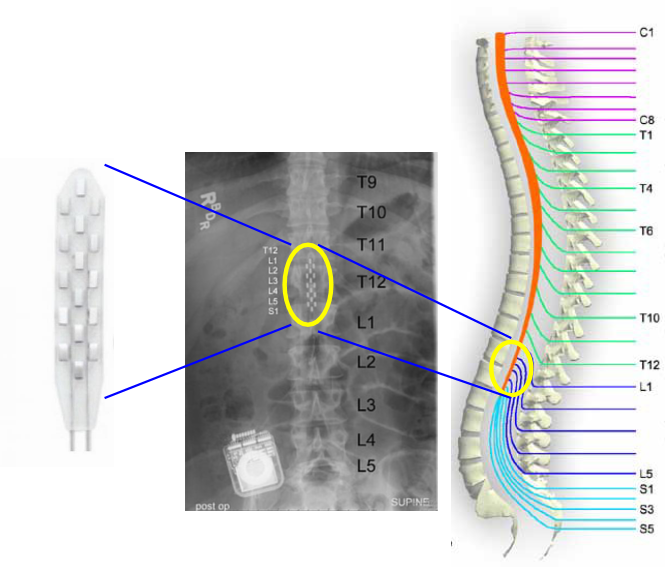
\includegraphics[width=2.5in]{figures/config1.png}
\end{center}
\column{0.45\textwidth}
\begin{center}
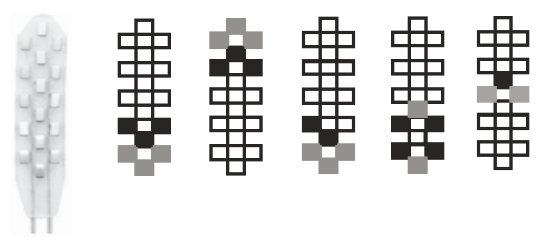
\includegraphics[width=2in]{figures/config2.png}
\vspace{2em}
\begin{itemize}
\item Electrode configurations are represented by points in $\mathbb{R}^4$
\vspace{1em}
\item Fit sq. exponential ARD kernel
\vspace{1em}
\item Run 300 iterations of each algorithm
\end{itemize}
\end{center}
\end{columns}
\end{frame}

\begin{frame}{Experiment 2: Spinal cord therapy}
\begin{columns}[c]
\column{0.55\textwidth}
\begin{center}
\setlength\figurewidth{2.5in}
\setlength\figureheight{1.7in}
\uncover<1->{
\begin{tikzpicture}

\begin{axis}[
title={{\footnotesize stop}},
title style={yshift=-1em},
tick label style={font=\footnotesize},
label style={font=\footnotesize},
width=\figurewidth,
height=\figureheight,
xmin=-0.5, xmax=2.5,
xtick={0, 1, 2},
xticklabels={{\footnotesize\algo}, {\footnotesize\localucb}, {\footnotesize\gpucb}},
%xticklabel style={
%  anchor=base
%},
ymin=0, ymax=100,
ytick={0, 25, 50, 75, 100},
%yticklabel style={rotate=90},
%ylabel=$\%$ of $\Rbeps(S_0)$,
major tick length=2pt,
axis lines*=left]

\addplot [
  ybar,
  bar width=0.4cm,
  cyan!50!black,
  line width=1pt,
  fill=cyan!75!black,
  solid
]
coordinates{
  (0,88.436346)
};

\addplot [
  ybar,
  bar width=0.4cm,
  lime!50!black,
  line width=1pt,
  fill=lime!70!black,
  solid
]
coordinates{
  (1,82.063342)
};

\addplot [
  ybar,
  bar width=0.4cm,
  orange!60!black,
  line width=1pt,
  fill=orange!85!black,
  solid
]
coordinates{
  (2,30.847086)
};

\addplot [
  only marks,
  mark=empty,
  darkgray,
  solid,
  error bars/.cd,
  error bar style={line width=1pt},
  y dir=both,
  y explicit
]
coordinates{
  (0,88.436346) +- (2*4.430386, 2*4.430386)
  (1,82.063342) +- (2*4.201586, 2*4.201586)
  (2,30.847086) +- (2*0.861908, 2*0.861908)
};

\end{axis}

\end{tikzpicture}
\\[0.5em]
}
\uncover<2->{
\begin{tikzpicture}

\begin{axis}[
title={{\footnotesize non-stop}},
title style={yshift=-1em},
tick label style={font=\footnotesize},
label style={font=\footnotesize},
width=\figurewidth,
height=\figureheight,
xmin=-0.5, xmax=2.5,
xtick={0, 1, 2},
xticklabels={{\footnotesize\algo}, {\footnotesize\localucb}, {\footnotesize\gpucb}},
%xticklabel style={
%  anchor=base
%},
ymin=0, ymax=100,
ytick={0, 25, 50, 75, 100},
%yticklabel style={rotate=90},
%ylabel=$\%$ of $\Rbeps(S_0)$,
major tick length=2pt,
axis lines*=left]

\addplot [
  ybar,
  bar width=0.4cm,
  cyan!50!black,
  line width=1pt,
  fill=cyan!75!black,
  solid
]
coordinates{
  (0,88.118102)
};

\addplot [
  ybar,
  bar width=0.4cm,
  lime!50!black,
  line width=1pt,
  fill=lime!70!black,
  solid
]
coordinates{
  (1,81.768031)
};

\addplot [
  ybar,
  bar width=0.4cm,
  orange!60!black,
  line width=1pt,
  fill=orange!85!black,
  solid
]
coordinates{
  (2,100)
};

\addplot [
  only marks,
  mark=empty,
  darkgray,
  solid,
  error bars/.cd,
  error bar style={line width=1pt},
  y dir=both,
  y explicit
]
coordinates{
  (0,88.118102) +- (2*4.421779,2*4.421779)
  (1,81.768031) +- (2*4.193425,2*4.193425)
  (2,100) +- (2*0,2*0)
};

\end{axis}

\end{tikzpicture}

}
\end{center}
\column{0.45\textwidth}
\centering
\setlength\figurewidth{2.5in}
\setlength\figureheight{3.7in}
\uncover<3->{
\begin{tikzpicture}

\begin{axis}[
name=plot1,
anchor=above north west,
tick label style={font=\footnotesize},
label style={font=\footnotesize},
title={\footnotesize\algo},
title style={yshift=-1em},
width=\figurewidth,
height=\figureheight/3,
xmin=0.33, xmax=1.02,
xtick={0, 0.2, 0.4, 0.6, 0.8, 1},
ymin=0, ymax=0.21,
ytick=\empty,
yticklabels={,,},
ylabel near ticks,
ylabel shift=-5pt,
major tick length=2pt,
axis lines*=left]

%% \addplot[
%%   color=cyan!75!black,
%%   solid,
%%   line width=1.5pt,
%%   samples=30,domain=0:6
%% ]
\addplot[
  ybar,
  bar width=0.15cm,
  cyan!50!black,
  line width=1pt,
  fill=cyan!75!black,
  solid
]
coordinates{
(0.56, 0.05714285714285714)(0.6, 0.2)(0.64, 0.05714285714285714)(0.6799999999999999, 0.05714285714285714)(0.72, 0.17142857142857143)(0.76, 0.08571428571428572)(0.8, 0.11428571428571428)(0.84, 0.02857142857142857)(0.88, 0.0)(0.92, 0.05714285714285714)(0.96, 0.14285714285714285)(1.0, 0.02857142857142857)
};

\addplot [
  magenta!50!darkgray,
  line width=1pt,
  dashed
]
coordinates{
(0.52512774,0)(0.52512774,60)
};

\addplot [
  mark=diamond*,
  mark size=3,
  only marks,
  cyan!35!black
]
coordinates{
(0.75177565,0)
};

\end{axis}

\begin{axis}[
yshift=-1em,
name=plot2,
at=(plot1.below south west),
anchor=above north west,
tick label style={font=\footnotesize},
label style={font=\footnotesize},
title={\footnotesize\localucb},
title style={yshift=-1em},
width=\figurewidth,
height=\figureheight/3,
xmin=0.33, xmax=1.02,
xtick={0, 0.2, 0.4, 0.6, 0.8, 1},
ymin=0, ymax=0.21,
ytick=\empty,
yticklabels={,,},
ylabel near ticks,
ylabel shift=-5pt,
major tick length=2pt,
axis lines*=left]

%% \addplot[
%%   color=lime!70!black,
%%   solid,
%%   line width=1.5pt,
%%   samples=30,domain=0:6
%% ]
\addplot[
  ybar,
  bar width=0.15cm,
  lime!50!black,
  line width=1pt,
  fill=lime!70!black,
  solid
]
coordinates{
(0.56, 0.034482758620689655)(0.6, 0.13793103448275862)(0.64, 0.13793103448275862)(0.6799999999999999, 0.10344827586206896)(0.72, 0.13793103448275862)(0.76, 0.06896551724137931)(0.8, 0.10344827586206896)(0.84, 0.0)(0.88, 0.06896551724137931)(0.92, 0.10344827586206896)(0.96, 0.10344827586206896)(1.0, 0.0)
};

\addplot [
  magenta!50!darkgray,
  line width=1pt,
  dashed
]
coordinates{
(0.52512774,0)(0.52512774,1)
};

\addplot [
  mark=diamond*,
  mark size=3,
  only marks,
  lime!35!black
]
coordinates{
(0.75088457,0)
};

\end{axis}

\begin{axis}[
yshift=-1em,
name=plot3,
at=(plot2.below south west),
anchor=above north west,
tick label style={font=\footnotesize},
label style={font=\footnotesize},
title={\footnotesize\gpucb},
title style={yshift=-1em},
width=\figurewidth,
height=\figureheight/3,
xmin=0.33, xmax=1.02,
xtick={0, 0.2, 0.4, 0.6, 0.8, 1},
ymin=0, ymax=0.21,
ytick=\empty,
yticklabels={,,},
ylabel near ticks,
ylabel shift=-5pt,
major tick length=2pt,
axis lines*=left]

%% \addplot[
%%   color=orange!85!black,
%%   solid,
%%   line width=1.5pt,
%% ]
\addplot[
  ybar,
  bar width=0.15cm,
  orange!60!black,
  line width=1pt,
  fill=orange!85!black,
  solid
]
coordinates{
(0.36, 0.017857142857142856)(0.4, 0.09821428571428571)(0.44, 0.05357142857142857)(0.48, 0.08035714285714286)(0.52, 0.0625)(0.56, 0.10714285714285714)(0.6, 0.044642857142857144)(0.64, 0.044642857142857144)(0.6799999999999999, 0.05357142857142857)(0.72, 0.03571428571428571)(0.76, 0.05357142857142857)(0.8, 0.05357142857142857)(0.84, 0.044642857142857144)(0.88, 0.03571428571428571)(0.92, 0.15178571428571427)(0.96, 0.044642857142857144)(1.0, 0.017857142857142856)
};

\addplot [
  magenta!50!darkgray,
  line width=1pt,
  dashed
]
coordinates{
(0.52512774,0)(0.52512774,0.7)
};

\addplot [
  mark=diamond*,
  mark size=3,
  only marks,
  orange!35!black
]
coordinates{
(0.66992681,0)
};

\end{axis}

\end{tikzpicture}

}
\end{columns}
\end{frame}

\begin{frame}{Conclusion}
\uncover<1->{
Recap
\vspace{0.5em}
\begin{itemize}
\item We formulated safe optimization using the concept of reachability
\vspace{0.5em}
\item We proposed SafeOpt, an algorithm with theoretical guarantees
\end{itemize}
}
\uncover<2->{
\vspace{2em}
What we skipped here
\vspace{0.5em}
\begin{itemize}
  \item Rigorous theoretical setup and analysis
  \vspace{0.5em}
  \item Another application: safe movie recommendation
\end{itemize}
\centering
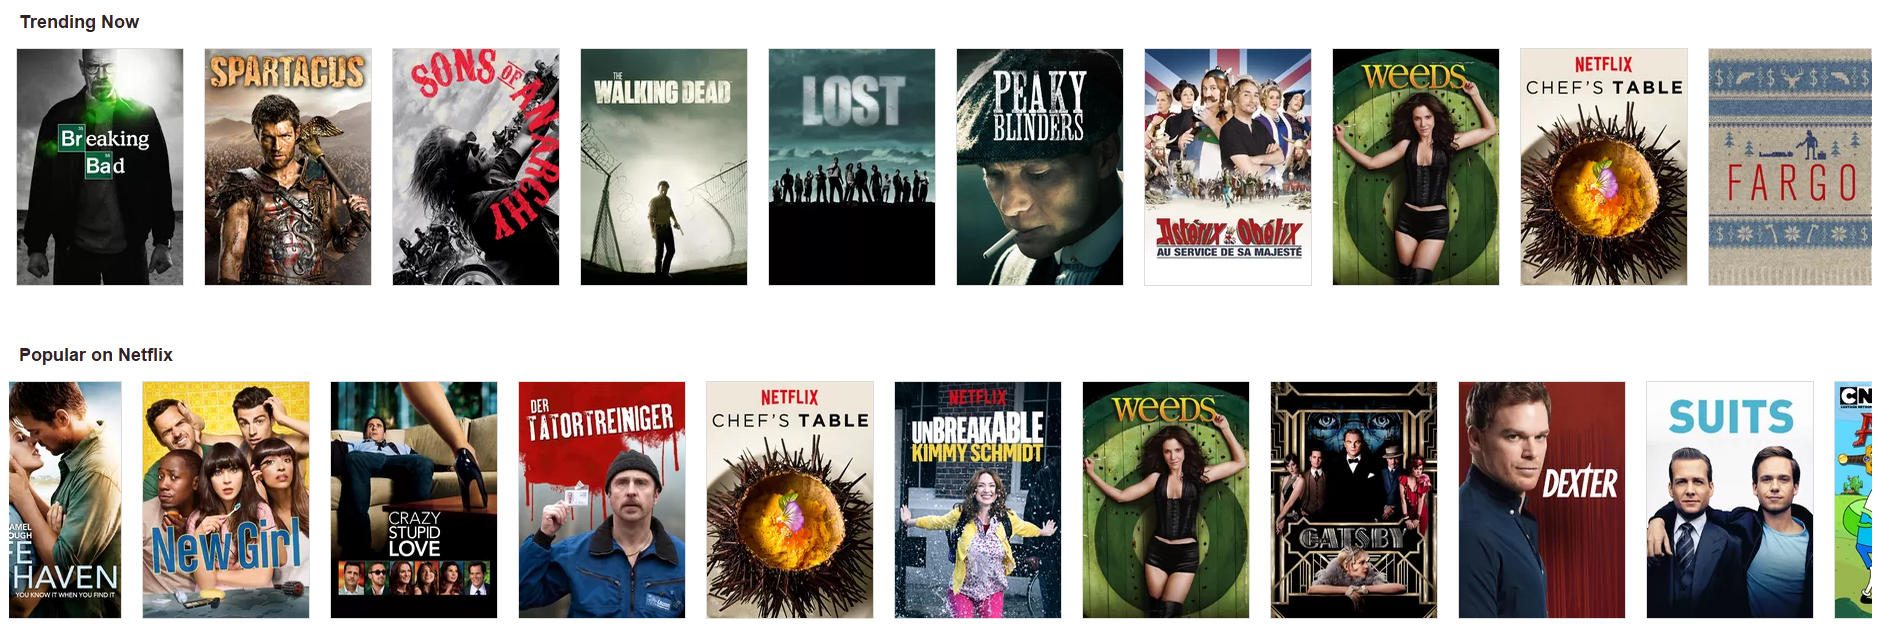
\includegraphics[width=3.5in]{figures/netflix.png}
}
\end{frame}

\end{document}
